% !Mode:: "TeX:UTF-8"
%%% Local Variables:
%%% mode: latex
%%% TeX-master: t
%%% End:

%面向对象的遥感影像的区间二型模糊聚类分割算法
\chapter{基于区间二型模糊聚类的遥感影像无监督分割方法}
\label{cha:chap03}

\section{引言}
\label{sec:chap03-1}
由于遥感影像数据具有同物异谱、同谱异物等固有的不确定性,结合模糊数学理论对不确定信息刻画的优点,模糊C-均值聚类(Fuzzy c-means clustering, FCM)分割方法被广泛应用到遥感影像分析中 \cite{bezdek1984fcm}。同时,随着遥感影像空间分辨率的提高,高分影像数据具有更多的信息多样性和复杂性,遥感影像聚类方法由传统的基于像元发展为面向对象的聚类分割。本章内容从遥感影像特征信息表达和目标地物类别关系两个角度来表征遥感影像分类中的不确定性信息。首先设计了三角形模糊集值信息表达模型来表征影像分割单元信息,其次提出一种新的区间值度量方法计算两个三角形模糊集值数据的相异性,最后,改进了已有的二型模糊集合聚类分割方法来对影像数据建模,以刻画遥感影像数据的不确定性  \footnote{本章部分内容来自作者2018年发表于 SCI 期刊 \textit{Computers \& Geosciences} 上的文章 \cite{jiang2018enhanced}。 }。
%\footnote{注:本章部分内容来自本文作者2018年发表于《Computers \& Geosciences》 SCI期刊的文章} hh

\begin{figure}[htbp]
    \centering
    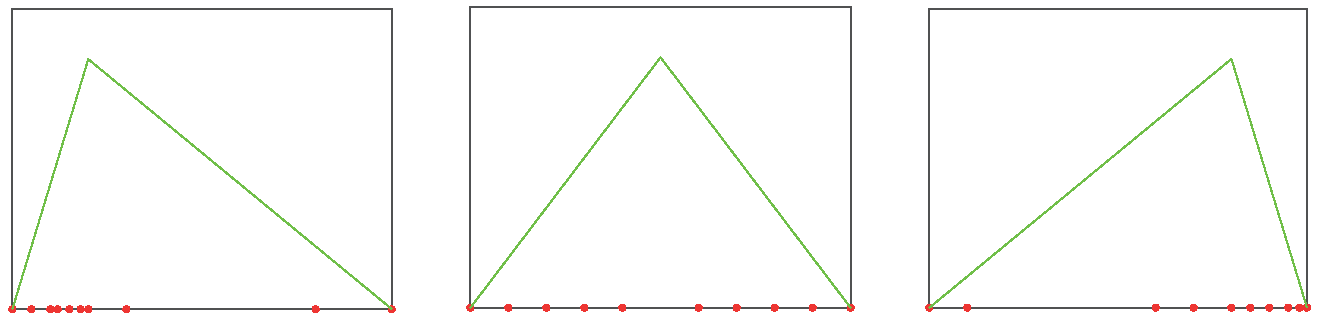
\includegraphics[width=0.9\textwidth]{figures/compare_distribution}
    \caption{区间值相同但分布不同的数据比较}
    \label{fig:compare_distribution}
\end{figure}

\section{三角形模糊集值建模与相似性度量}
\label{sec:chap03-2}
当前,面向对象分割方法中对影像单元多采取均值数据建模 \cite{yu2012method} 和区间值数据建模 \cite{he2016remote} 。然而,这两种信息表达模型无法区分具有相同均值和区间值但内部分布不一致的分割单元。如图 \ref{fig:compare_distribution} 所示,每组模拟数据内的点集可以看作一个影像分割单元像素点集合,具有相同的均值和区间值的影像单元内像素点的分布差异明显。

模糊集(Fuzzy sets, FS) 是 Zadeh 教授 1965年提出的概念,通过建立适当的隶属度函数(Membership function, MF)来描述对象的不确定性 \cite{zadeh1965fuzzy}。 常见的隶属度函数有:三角形MF,梯形MF,截断高斯MF和钟形MF等。 FS 最常用和最基本的 MF 是三角形MF。 因此,文中利用三角形模糊集来定义三角形模糊集值数据模型。

\begin{definition}
    \label{define1}
    三角形模糊集值(Triangular Fuzzy Set Valued, TFSV)模型的定义
\end{definition}
三角形模糊集值数据由以下三个关键参数组成:$(a^-,0)$,$(a^m,1)$ 和 $(a^+,0)$。如图~\ref{fig:tfs} 所示,  几何上,$(a^-,0)$ 和 $(a^+,0)$ 组成三角形MF的下边缘;代数上,$(a^-,0)$ 和 $(a^+,0)$ 形成一个区间值,确保一定的变化范围。$(a^m,1)$是TFSV 数据的顶点,表征 FS 的最高置信度。
\begin{figure}[htbp]
    \centering
    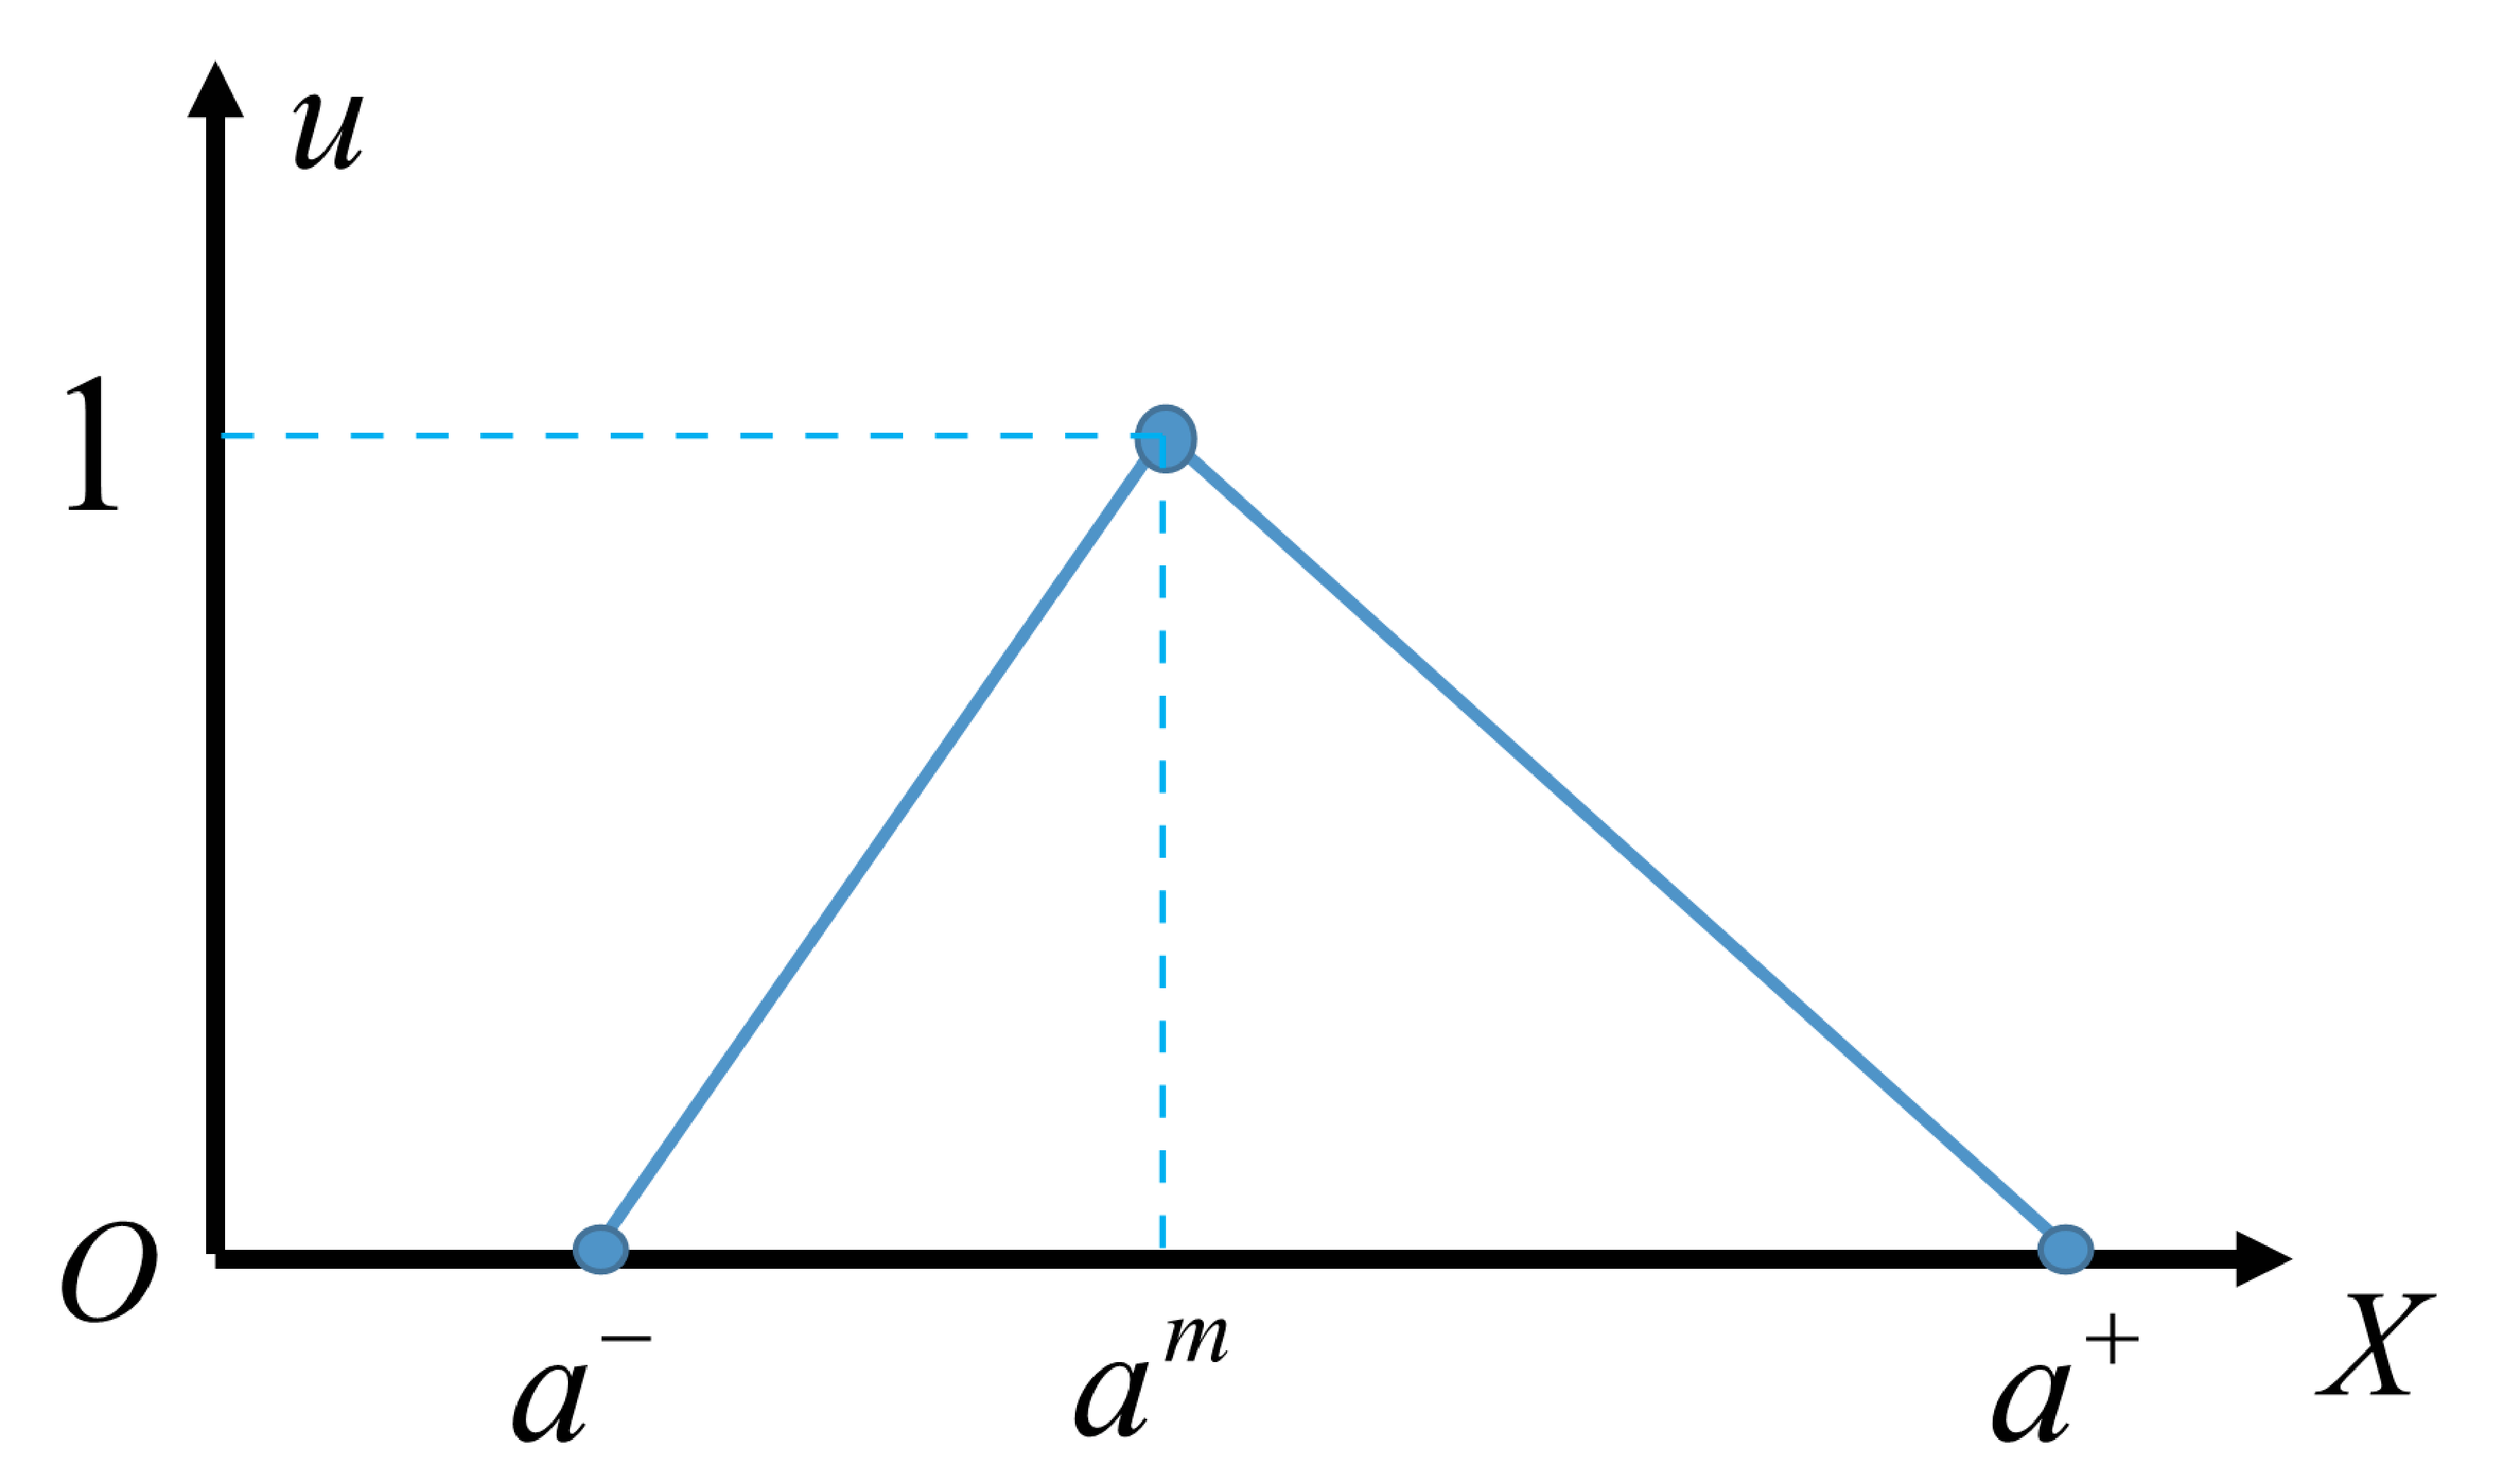
\includegraphics[width=0.5\textwidth]{figures/tfs}
    \caption{三角形模糊集 $\tilde{A}$ 示意图}
    \label{fig:tfs}
\end{figure}

聚类是根据某种相似性或距离将相似的对象聚为一类的无监督学习方法,相似性度量是聚类的核心要素。对于两个TFSV 数据$\tilde{A}$ 和 $\tilde{B}$,常见的相似性度量方法有以下几种:
\begin{enumerate}[(1)]
    \item 欧式距离(Euclidean distance)

          \begin{equation}
              \label{equ:eucliden}
              d_E(\tilde{A}, \tilde{B}) = \sqrt{\sum_{x \in X} |\tilde{A}(x)-\tilde{B}(x)|^2 }, x \in X
          \end{equation}
          $\tilde{A}$ 和 $\tilde{B}$ 的欧式距离 $d_E(\tilde{A}, \tilde{B})$ 被看作是集合对应元素差值平方和的平方根。
    \item 城市距离(City-block distance)

          \begin{equation}
              \label{equ:cityblock}
              d_C(\tilde{A}, \tilde{B}) = \sum_{x \in X}|\tilde{A}(x)-\tilde{B}(x)| , x \in X
          \end{equation}
          $\tilde{A}$ 和 $\tilde{B}$ 的城市距离 $d_C(\tilde{A}, \tilde{B})$ 被看作是集合对应元素差值绝对值的和。
          %  \item 切比雪夫距离(Tchebyshev distance)

          %        \begin{equation}
          %            \label{equ:tchebyshev}
          %            d_T(\tilde{A}, \tilde{B}) = \sqrt[\infty]{\int_X |\tilde{A}(x)-\tilde{B}(x)|^\infty dx }, x \in X
          %        \end{equation}
          %        $\tilde{A}$ 和 $\tilde{B}$ 的切比雪夫距离 $d_T(\tilde{A}, \tilde{B})$ 被看作是集合对应元素差值积分的一个极限值。
    \item 豪斯多夫距离(Hausdorff distance)

          豪斯多夫距离最开始为区间或普通集合设计,两个普通集合 $A$ 与 $B$ 的豪斯多夫距离为:
          \begin{equation} \label{eq:haus1}
              d_H(A, B) = \max \Big  \lbrace \sup_{a \in A} \inf_{b \in B} \abs{a-b}, \sup_{b \in B} \inf_{a \in A} \abs{a-b} \Big  \rbrace
          \end{equation}
          将其推广到模糊集,可以考虑模糊集 $\tilde{A}$ 和 $\tilde{B}$的一个 $\alpha-cut$ 截集  \cite{zadeh1965fuzzy} $d_H^{\alpha} (\tilde{A}, \tilde{B})$,则有:
          \begin{equation}\label{eq:haus_alpha}
              \begin{split}
                  d_H^{\alpha} (\tilde{A}, \tilde{B}) = \max \Big \lbrace \sup_{a \in \tilde{A_{\alpha}}} \inf_{b \in \tilde{B_{\alpha}}} \abs{a-b}, \sup_{b \in \tilde{B_{\alpha}}} \inf_{a \in \tilde{A_{\alpha}}}
                  \abs{a-b} \Big \rbrace
              \end{split}
          \end{equation}
          其中,$\inf$ 和 $\sup$ 分别表示取集合的最大下界和最小上界。模糊集是度量空间的非空紧致和有限子集,所以等式~\ref{eq:haus_alpha} 中的 $\inf$ 和 $\sup$ 操作可分别替换为 $\min$ 和 $\max$ 操作, 即
          \begin{equation}\label{eq:haus_alpha2}
              \begin{split}
                  d_H^{\alpha} (\tilde{A}, \tilde{B}) = \max \Big \lbrace \max_{a \in \tilde{A_{\alpha}}} \min_{b \in \tilde{B_{\alpha}}} \abs{a-b}, \max_{b \in \tilde{B_{\alpha}}} \min_{a \in \tilde{A_{\alpha}}} \abs{a-b} \Big \rbrace
              \end{split}
          \end{equation}
          然后对 $\tilde{A}$ 和 $\tilde{B}$ 所有可能的$\alpha-cut$ 截集积分,就可得到模糊集 $\tilde{A}$ 和 $\tilde{B}$的豪斯多夫距离:
          \begin{equation}\label{eq:haus2}
              \begin{split}
                  d_H(\tilde{A}, \tilde{B}) = \int_0 ^1 d_H^{\alpha} (\tilde{A}, \tilde{B}) d \alpha = \int_0 ^1 \max \Big \lbrace \max_{a \in \tilde{A_{\alpha}}} \min_{b \in \tilde{B_{\alpha}}} \abs{a-b}, \max_{b \in \tilde{B_{\alpha}}} \min_{a \in \tilde{A_{\alpha}}} \abs{a-b} \Big \rbrace  d \alpha
              \end{split}
          \end{equation}

\end{enumerate}



那么,如何选择合适的距离来度量两个模糊集的相似性呢?对于模糊集 $\tilde{A}$ 和 $\tilde{B}$,如图~\ref{fig:set_location} 所示,我们考虑在同一坐标系内, $\tilde{A}$ 和 $\tilde{B}$ 只存在三种位置关系:相交、包含和不相交。

\begin{figure}[!htb]
    \centering
    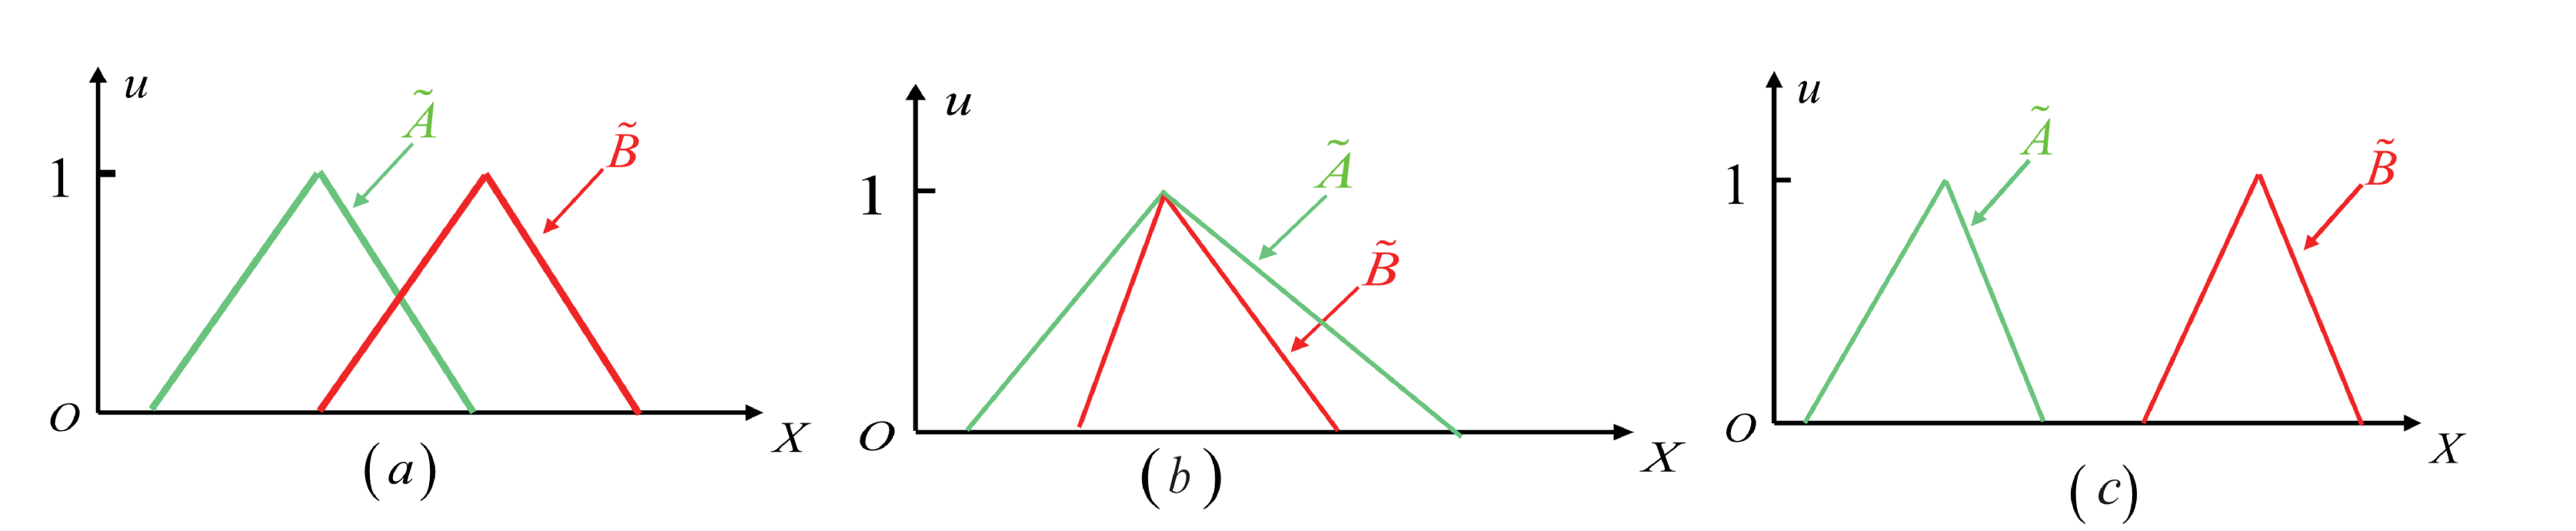
\includegraphics[width=0.9\textwidth]{figures/set_location}
    \caption{$\tilde{A}$ 和 $\tilde{B}$ 位置关系示意图。 (a)相交; (b)$\tilde{A}$ 包含集合$\tilde{B}$;  (c)不相交.}
    \label{fig:set_location}
\end{figure}

为了比较各种位置关系下两个模糊集间上述各种距离的大小关系。文中设计以下实验:如图~\ref{fig:distance_compare}(a) 所示,$\tilde{B}$ 固定不动,将$\tilde{A}$ 沿$\textbf{X}$ 轴从左向右移动,分别计算各相对位置下$\tilde{A}$ 和$\tilde{B}$ 对应位置的距离。结果如图~\ref{fig:distance_compare}(b) 所示(图中$0-cut$ 和$1-cut$ 截集的豪斯多夫距离后面会讨论),$\tilde{A}$ 位于$(a,b)$ 区间内时,$\tilde{A}$ 和$\tilde{B}$ 相交,以上四种距离均可度量$\tilde{A}$ 和$\tilde{B}$ 的相似性。 然而,在两者不相交时(图中$\tilde{A}$ 位于$(-\infty, a)$ 和$(b,+\infty)$ 区间内)无论$\tilde{A}$ 和$\tilde{B}$ 相距多远,欧式距离和城市距离均为一固定常量,只有豪斯多夫距离可以精确度量上述三种位置下两个模糊集的相似性。

\begin{figure}[!htb]
    \centering
    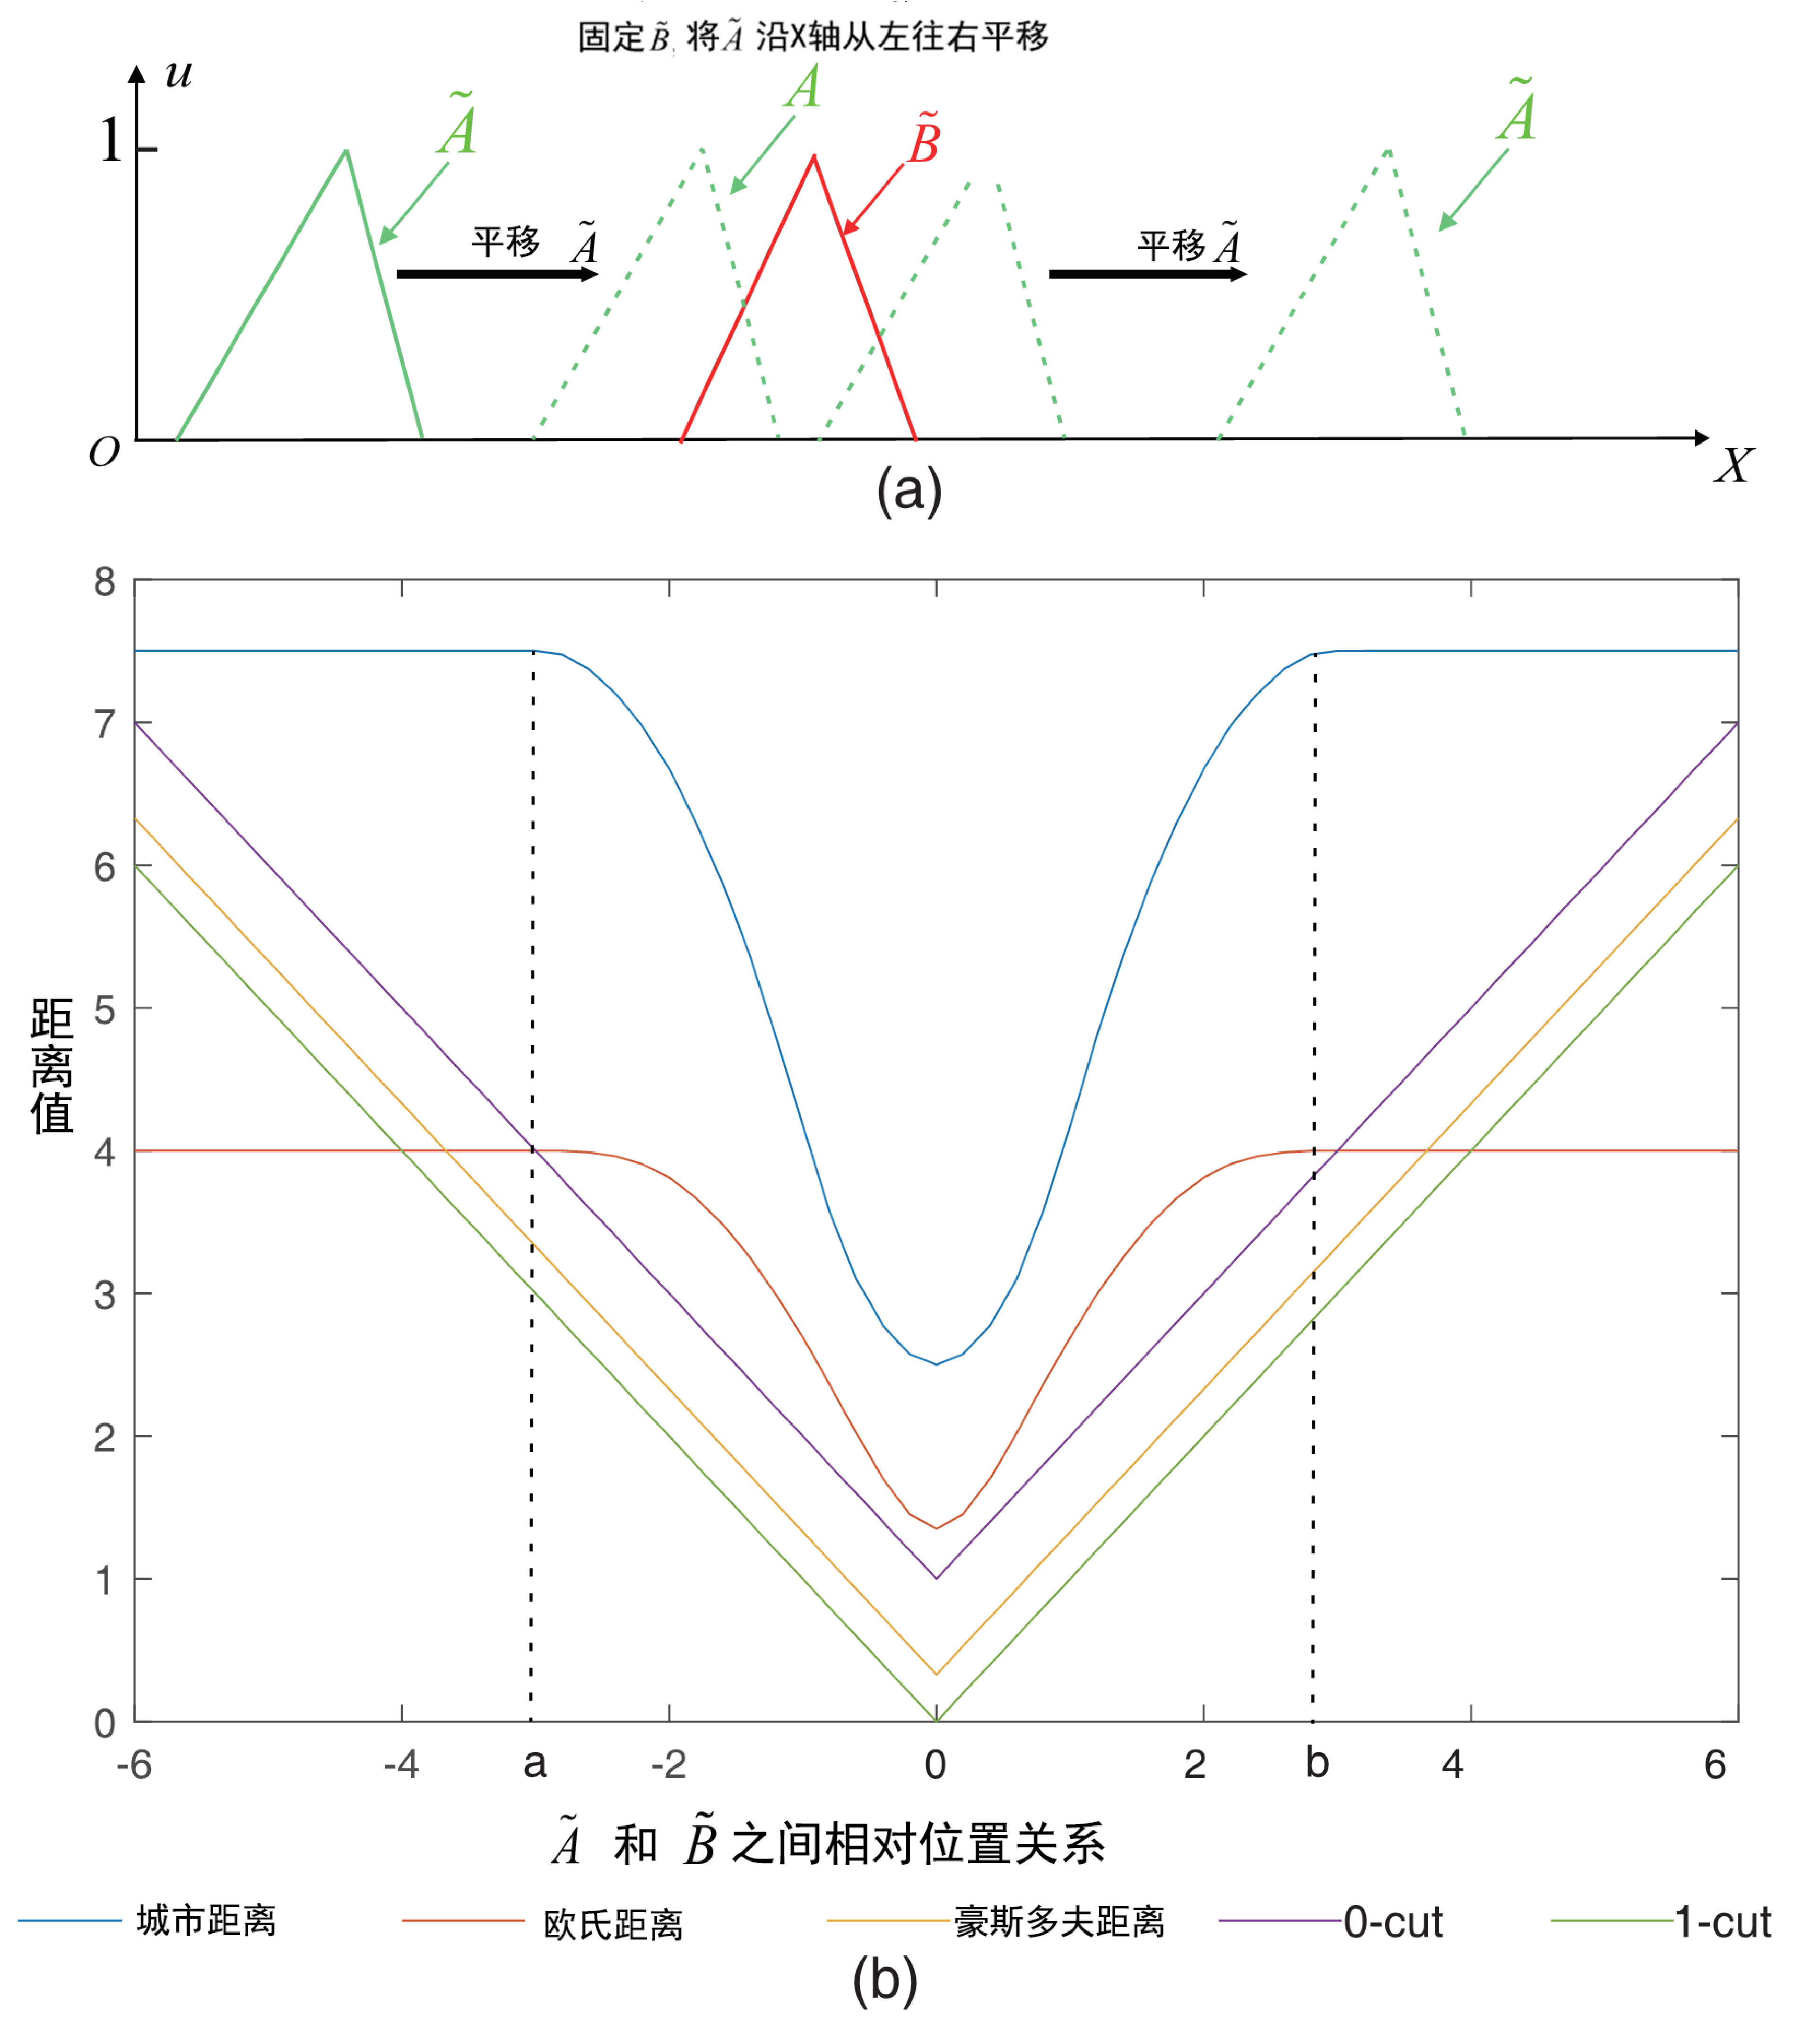
\includegraphics[width=0.9\textwidth]{figures/distance_compare}
    \caption{不同位置下,$\tilde{A}$ 和 $\tilde{B}$ 两者间各种距离比较图。}
    \label{fig:distance_compare}
\end{figure}

然而,计算两个模糊集之间的豪斯多夫距离具有较高的计算复杂度,导致其在模糊聚类迭代更新中难以适用。另外,Zadeh 教授在可能性分布理论\cite{zadeh1978fuzzy} 中提到: 模糊集作为一个弹性约束值, 若使用区间距离度量, 而不是一个单一固定值来度量两个模糊集间相似性可以获取产生更高的识别能力。因此, 文中尝试引入一种新的基于豪斯多夫距离的区间距离度量方法来度量三角形模糊集的相似性。

首先,考虑模糊集合的特性, 文献 \cite{zadeh1978fuzzy} 中定义了模糊集的$\alpha-cut$ 截集并提出了模糊集的$\alpha-cut$ 截集表现定理,其中提到任何模糊集都可以由它指定的$\alpha-cut$ 截集来表示。在所有的截集中,有两个截集是最重要与最具有代表性的,它们就是$0-cut$ 和$1-cut$ 截集,分别代表模糊集和的支撑集和置信集合。模糊集$\tilde{A}$ 的支持集$0-cut$ 包含$\tilde{A}$ 中非零的所有元素,体现了模糊集的可能性;而$\tilde{A}$ 的置信集$1-cut$ 包含元素的隶属度均为$1$,这表明$1-cut$ 截集中所有元素都有最高的隶属度和置信度,体现了模糊集的必要性。此外,最近一些关于$\alpha-cut$ 截集的研究对任一模糊集,仅使用$0-cut$ 和$1-cut$ 截集就可近似拟合模糊集的质心;此外,任意其他$\alpha -cut$ 截集$ (0 \leq \alpha \leq 1)$ 都可以表示为$0-cut$ 和$1-cut$ 截集的广义线性组合\cite{liu2008efficient}。

根据公式\ref{eq:haus_alpha2}, 我们分别可以获得$\tilde{A}$ 和$\tilde{B}$ 的$0-cut$ 和$1-cut$ 的豪斯多夫距离为$d_H^{0} (\tilde{A}, \tilde{B})$ 和 $d_H^{1} (\tilde{A}, \tilde{B})$。基于上面提到的可能性分布理论和模糊集的$\alpha-cut$ 截集表现定理,我们可以定义两个三角形模糊集间$\tilde{A}$ 和$\tilde{B}$ 间一种新的区间值距离$d_I (\tilde{A}, \tilde{B})$ 为下式:
\begin{equation}\label{eq:interval}
    \begin{split}
        d _{I} (\tilde{A},\tilde{B}) = [\min \lbrace d_0 (\tilde{A},\tilde{B}),d_1(\tilde{A},\tilde{B}) \rbrace, \max \lbrace d_0(\tilde{A},\tilde{B}), d_1 (\tilde{A},\tilde{B}) \rbrace ]
    \end{split}
\end{equation}
图~\ref{fig:distance_compare} 中的结果($0-cut$ 和$1-cut$)也表明$d _{I} (\tilde{A},\tilde{B})$ 能够度量两个模糊集不相交时的相似性;另外,还可以看出文中新定义的距离$ d _{I} (\tilde{A},\tilde{B})$ 是$ d _{H} (\tilde{A},\tilde{B})$的弹性膨胀,即有:
\begin{equation}\label{eq:expand_in}
    \begin{split}
        d _{H} (\tilde{A},\tilde{B}) \in d _{I} (\tilde{A},\tilde{B})
    \end{split}
\end{equation}
公式~\ref{eq:expand_in}的证明步骤由于篇幅过大,可参考本文作者已发表文章\cite{jiang2018enhanced} 的附录一。

一个相似性度量能够定位为距离,当且仅当其能满足距离度量三个条件,即非负性、对称性和三角不等式。假定$\tilde{A}$、$\tilde{B}$ 和$\tilde{C}$是任意三个三角形模糊集,则需要满足以下特性:
\begin{enumerate}[(1)]
    \item \textsl{非负性}: $d_I(\tilde{A}, \tilde{A}) = 0$
    \item\textsl{对称性}: $d_I(\tilde{A}, \tilde{B}) = d_I(\tilde{B}, \tilde{A})$
    \item  \textsl{三角不等式}: $d_I(\tilde{A}, \tilde{C}) \leq d_I(\tilde{A}, \tilde{B}) + d_I(\tilde{B}, \tilde{C})$
\end{enumerate}
证明过程较复杂且非文章研究重点,可参考本文作者已发表文章\cite{jiang2018enhanced} 的附录二。

综上所述,本节针对面向对象分割单元定义了TFSV 数据模型,同时,结合模糊集与可能性分布定理特性,针对新提出的TFSV 数据类型,本文新提出了一种区间值的距离度量方法,来度量两个TFSV 数据间的相似性。


\section{面向对象的改进型区间二型模糊遥感影像聚类方法}
\label{sec::chap03-3}


\subsection{算法整体框架}
\label{subsec::chap03-3}
本章提出基于三角形模糊集值的区间二型模糊聚类方法(Triangular Fuzzy Set Valued Interval Type 2 Fuzzy Clustering Method, TFSV-IT2FCM)主要用于提高高分辨率遥感影像无监督聚类分割精度。图~\ref{fig:framework} 展示了该面向对象分类方法的总体处理流程,具体可分为以下几点:

\begin{enumerate}[Step 1:]
    \item 影像分割与对分割单元的TFSV 数据建模

          高分影像被分割为具有同质性的像素单元集合.对分割单元提取特征,并构建 TFSV 模型;
    \item 模糊聚类分析

          使用TFSV-IT2FCM 算法对高分影像分割单元的TFSV 模型数据聚类,IT2FCM 算法的距离度量使用文中新提出的区间距离$d_I$;
    \item 聚类结果的后处理

          使用类别组合方法对聚类分割的结果处理,得到高分影像最终得分割结果。
\end{enumerate}

\begin{figure}[htb]
    \centering
    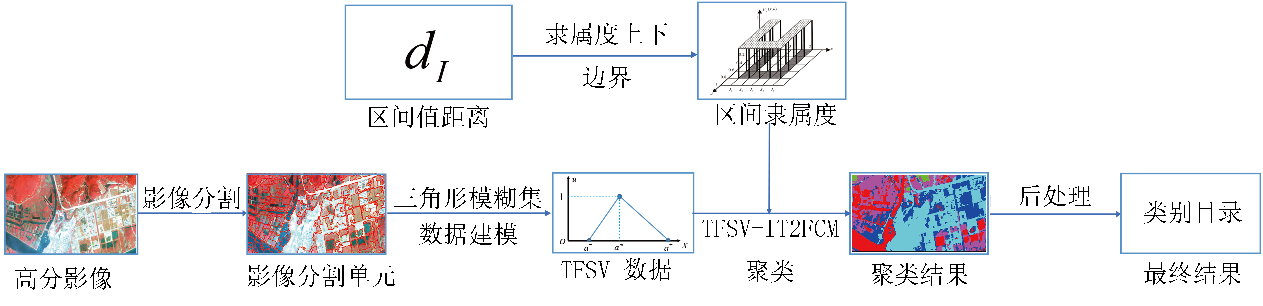
\includegraphics[width=1.0\textwidth]{figures/framework}
    \caption{面向对象的改进型区间二型模糊遥感影像聚类算法框架图}
    \label{fig:framework}
\end{figure}


\subsection{面向对象的TFSV 模型}
\label{subsec::chap03-3-1}

\subsubsection*{1.影像分割}
\label{subsec::chap03-3-1-1}

目前,遥感影像常用的像元分割算法包含基于分水岭的算法,基于直方图的方法和聚类方法等\cite{roerdink2000watershed}。简单线性迭代聚类(SLIC)算法具有高计算效率和可选数量的分段单元\cite{achanta2012slic},因此本章使用SLIC 超像素分割算法提取遥感影像的分割单元。 SLIC 算法的关键步骤如下:
\begin{enumerate}[(I)]
    \item 计算遥感影像梯度获取影像梯度图;
    \item 初始化梯度图中的聚类中心;
    \item 将遥感影像从SPOT5 格式转换为CIELAB 颜色空间计算像元间的相似度;
    \item 使用SLIC 算法对CIELAB 彩色图像进行分割,以获得影像同质性分割单元。
\end{enumerate}

对高分影像$\bm{I}$ ,使用SLIC 分割算法获得影像分割单元 $\bm{SS}$,为:
\begin{equation}\label{eq:image_ss}
    \begin{split}
        \bm{SS} = \lbrace \bm{B_1}, \bm{B_2},\bm{\cdots}, \bm{B_n} \rbrace
    \end{split}
\end{equation}
其中$\bm{B_i}(1 \leq i \leq n)$ 表示第$i$ 个分割单元,$n$ 表示分割单元的总数。 $\bm{B_i}(i=1,2,\cdots, n)$ 是一个$j \times p$ 矩阵,其中$j$ 表示每个波段包含的像素数目,$p$ 表示图像通道数。


\subsubsection*{2.影像单元的TFSV 数据建模}
尽管文献\cite{he2016remote} 中已经证明:对于影像分割单元,区间值的特征比均值特征更有效,但是影像分割单元的不确定性不能被充分的表达。因此,文中使用定义 \ref{define1} 的TFSV 数据模型$\bm{\tilde{A_i}}$  来提取影像单元$\bm{B_i}$ 的特征:
\begin{enumerate}[ 1)]
    \item 基于影像分割单元$\bm{B_i}$内像素的均值和方差特性,可以获得一个$p$ 维的区间值向量,记为$\bm{X_i}$,如下:
          \begin{equation}\label{eq:eq-1}
              \bm{X_i} = [\bm{X_{i}^{down}},\bm{X_i^{up} }] = [\max{\lbrace 0,\bm{\mu_i} - \alpha \times \bm{\sigma_i} \rbrace}, \bm{\mu_i} + \alpha \times \bm{\sigma_i}]
          \end{equation}

          其中$\bm{\mu_i} = [\mu_{1}, \mu_2,\cdots,\mu_p]^T$,$\bm{\sigma_i} = [\sigma_{1},\sigma_2,\cdots,\sigma_p] ^T$ 是第$i$个分割单元$\bm{B_i}$ 的均值和方差,$\alpha$ 是控制区间值大小的超参数,$p$ 是遥感影像的波段数。
    \item 分割单元是邻近同质像素点的集合,基于统计学特性,等式\ref{eq:eq-1} 中的向量$\bm{X_i} = [\bm{X_{i}^{down}},\bm{X_i^{up} }]$ 除了少数异常点外包含分割单元$\bm{B_i}$中的绝大部分点。因此,从$\bm{X_i}$ 中导出参数 $(\bm{X_{i}^{down}},0)$ 和$(\bm{X_i^{up}},0)$来构造$\bm{\tilde{A_i}}$ 的底边。
    \item $\bm{\tilde{A_i}}$ 的顶点由$(\bm{med_i},1)$ 组成。因中值不受极值的影响,并且对噪声点和异常值具有很高的鲁棒性,这里$\bm{med_i}$ 取$\bm{B_i}$ 的中值。
\end{enumerate}


类似地,影像的每个分割单元都可以被表征为一个 TFSV 数据模型,分割单元的集合$\bm{SS} = \lbrace \bm{B_1}, \bm{B_2},\bm{\cdots}, \bm{B_n} \rbrace$ 可以被表示为:

\begin{equation}\label{eq:eq-2}
    \bm{SS} \to \lbrace \bm{\tilde{A_1}}, \bm{\tilde{A_2}},\bm{\cdots}, \bm{\tilde{A_n}} \rbrace
\end{equation}

其中$\bm{SS}$ 是一个$n \times p$ 矩阵,$\bm{\tilde{A_i}}$ 是$\bm{B_i}$ 对应的$p$ 维TFSV 数据,$n$ 表示分割单元的数目。


\subsection{基于TFSV 数据模型的面向对象模糊聚类方法}
\label{subsec::chap03-3-2}


\subsubsection*{1.区间二型模糊隶属度}
\label{subsec::chap03-3-3-2-1}
区间二型模糊聚类算法(Interval type 2 fuzzy clustering method, IT2FCM) 使用一个区间值来表示隶属度值。文献\cite{hwang2007uncertain} 中使用两个模糊化指数$m_1$ 和$m_2$ 得到区间二型隶属度函数(Interval type 2 membership function,IT2MF) 的上界和下界,从而将一型模糊集(Type 1 fuzzy sets, T1FS) 扩展为二型模糊集(Type 2 fuzzy sets, T2FS)。然而,IT2FCM 算法对模糊指数$m_1$ 和$m_2$ 的取值敏感。与传统FCM 算法相比,不恰当的$m_1$ 和$m_2$ 取值会导致更差的实验结果。因此,基于公式~\ref{eq:interval} 中新定义的区间值距离度量,类似FCM 算法,本文仅使用一个模糊指数$m$ 来表达IT2MF。


\begin{figure}[htbp]
    \centering
    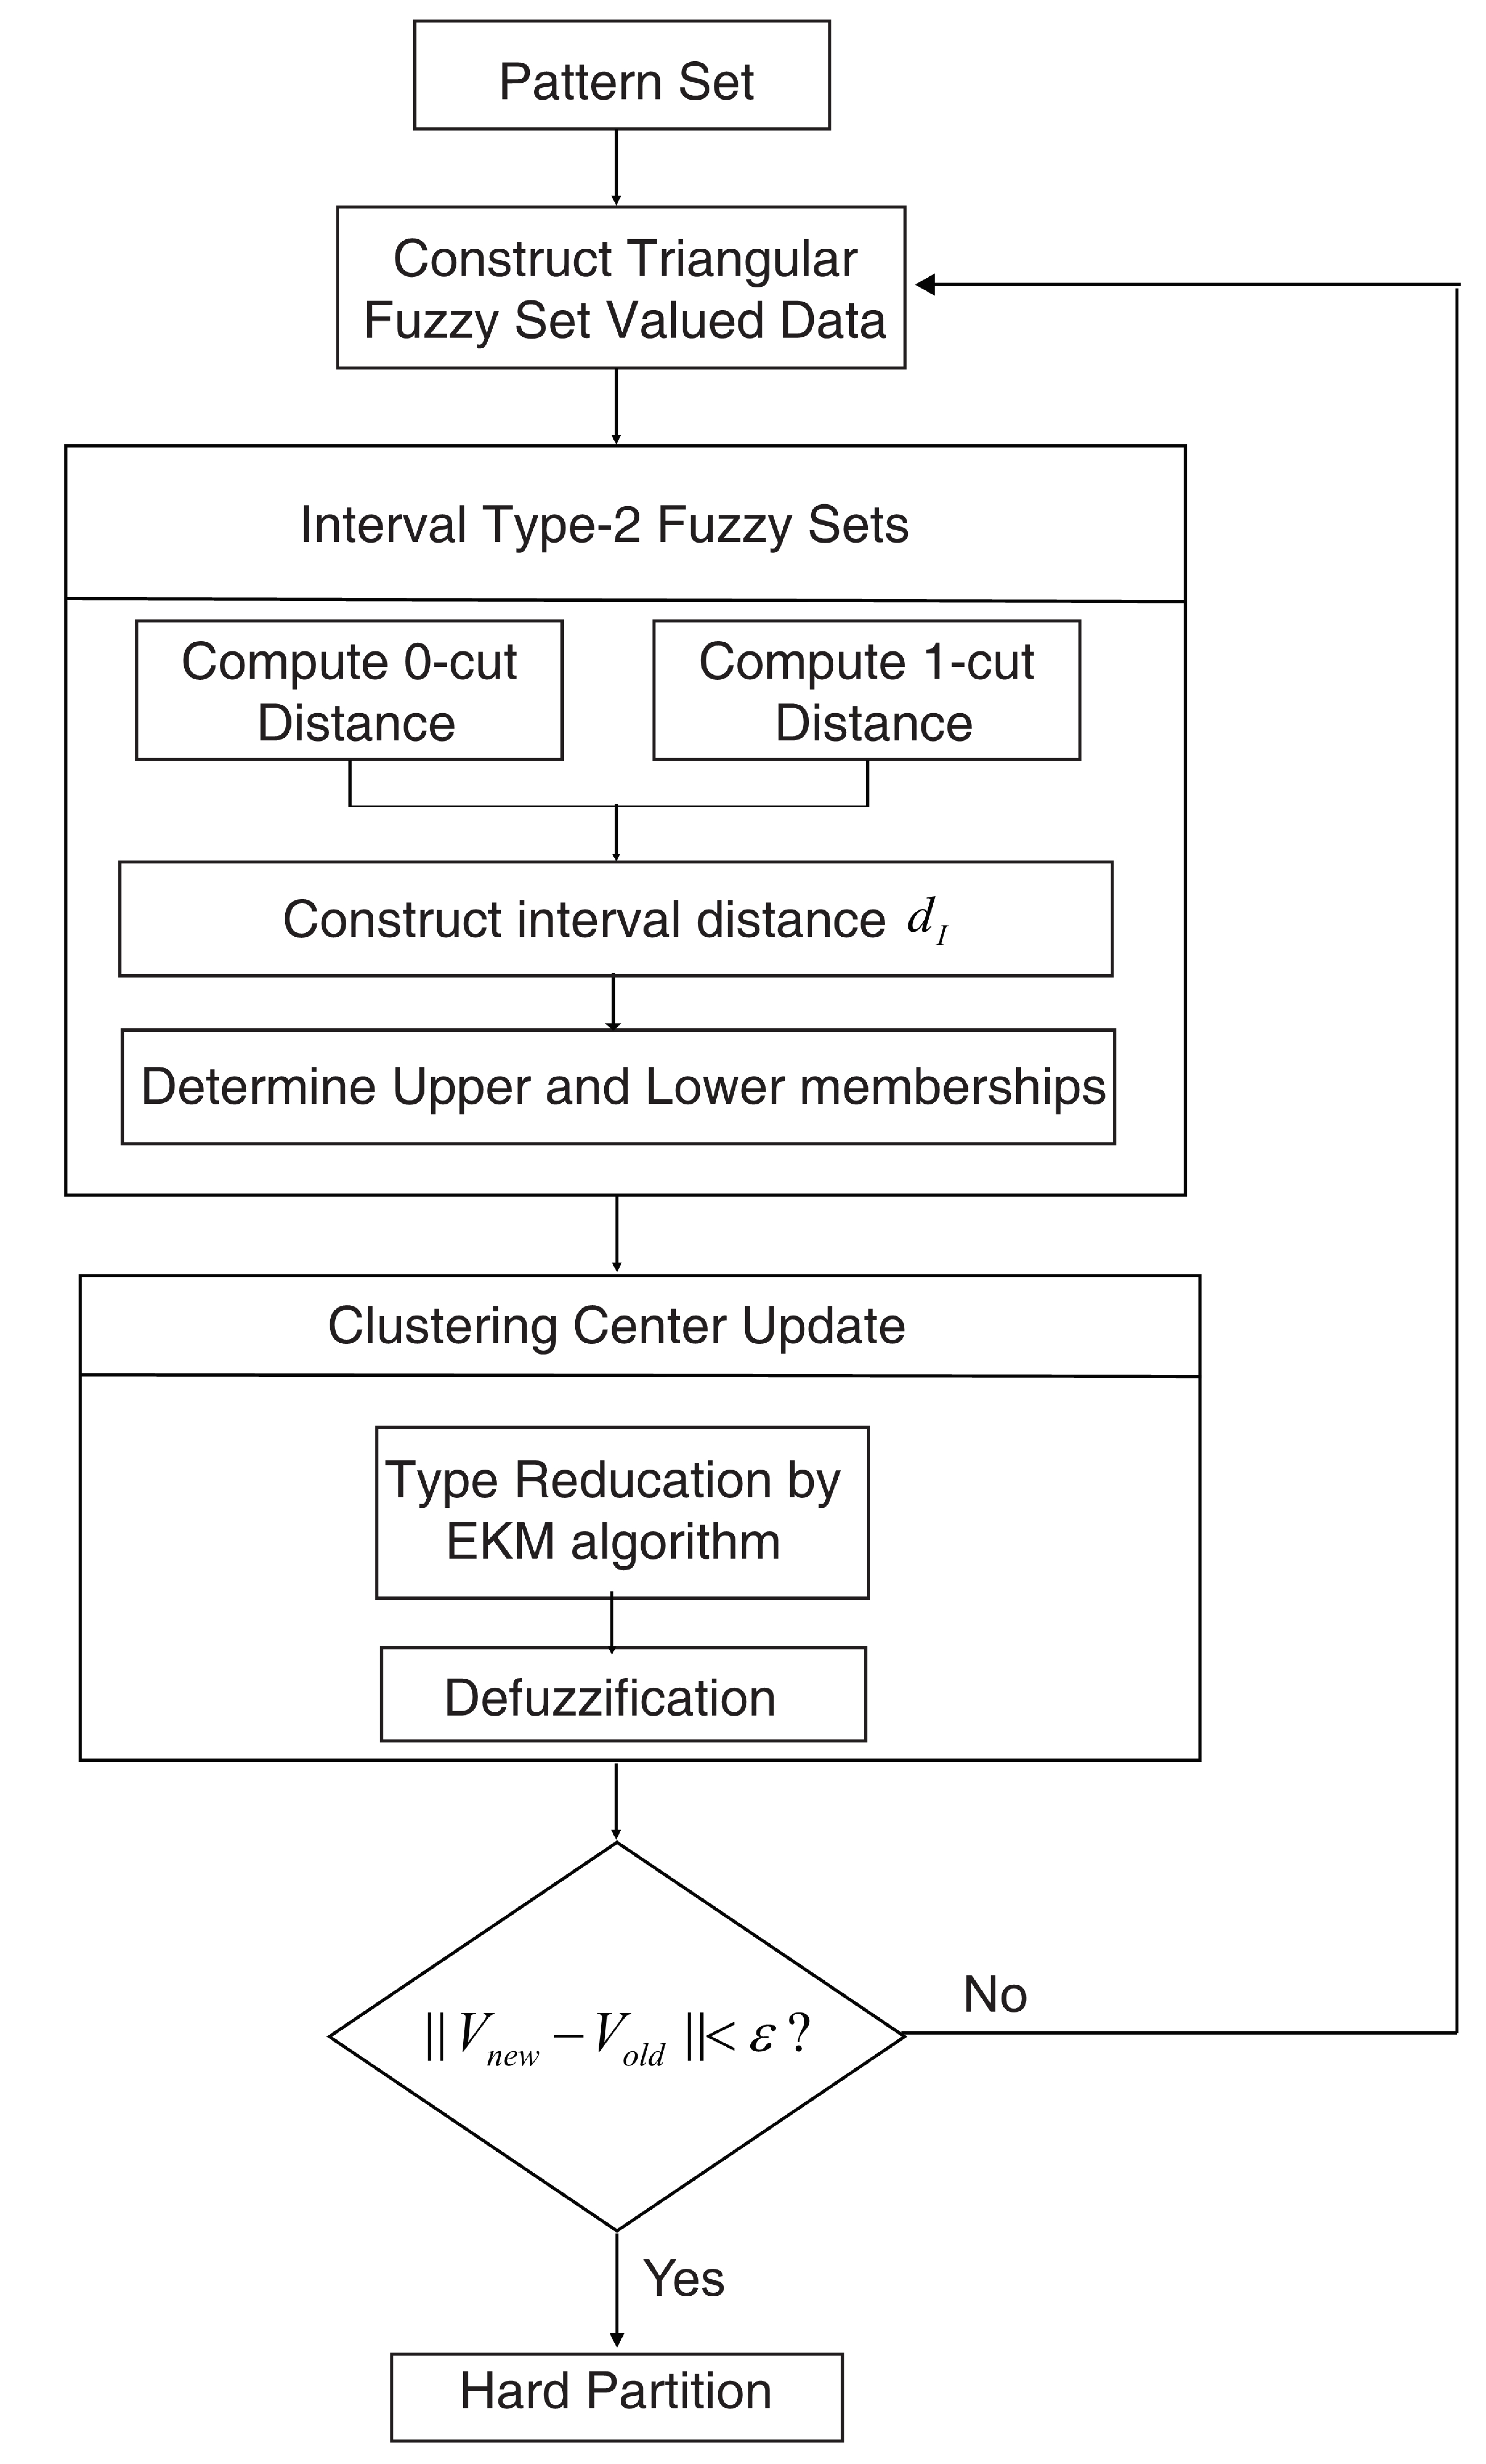
\includegraphics[width=0.8\textwidth]{figures/tfsvit2}
    \caption{TFSV-IT2FCM 算法流程图}\label{fig:tfsvit2}
  \end{figure}

假定样本$\bm{\tilde{X}} = (\tilde{X_1}, \tilde{X_2},\cdots, \tilde{X_p})^T$ 和聚类中心$\bm{\tilde{V}} = (\tilde{V_1}, \tilde{V_2},\cdots, \tilde{V_p})^T$ 是两个形如公式~\ref{eq:eq-2} 的$p$ 维TFSV 数据,其中$\tilde{X_i}$ $(1 \leq i \leq p)$ 是一个一维TFSV,由$(X_{i}^{down}, 0)$,$(X_{i}^{up}, 0)$和$(X_i^{med}, 1)$ 这三个参数构成;类似地,$\tilde{V_i}$ 由$(V_{i}^{down}, 0)$,$(V_{i}^{up}, 0)$ 和$(V_i^{med}, 1)$三个参数组成。$\tilde{X_i}$ 和$\tilde{V_i}$ 的$0-cut$ 和$1-cut$ 豪斯多夫距离分别为:

\begin{equation}\label{eq:eq-3}
    \begin{split}
        d_0 (\tilde{X_i}, \tilde{Y_{i}}) = \max \Big \lbrace \abs{X_i^{down} - Y_i^{down}}, \abs{X_i^{up} - Y_i^{up}} \Big \rbrace
    \end{split}
\end{equation}
和
\begin{equation}\label{eq:eq-4}
    \begin{split}
        d_1 (\tilde{X_i}, \tilde{V_{i}}) = \Big\lbrace |X_i^{med} - V_i^{med}| \Big\rbrace
    \end{split}
\end{equation}
$\tilde{X_i}$ 和$\tilde{V_{i}}$ 的区间值距离$d_{I} (\tilde{X_i}, \tilde{V_i})$ 即为:
\begin{equation}\label{eq:eq-5}
    \begin{split}
        d_{I} (\tilde{X_i}, \tilde{V_i}) = [\min \lbrace d_0 (\tilde{X_i}, \tilde{V_{i}}) , d_1 (\tilde{X_i}, \tilde{V_{i}}  \rbrace,\max  \lbrace d_0 (\tilde{X_i}, \tilde{V_{i}}) , d_1 (\tilde{X_i}, \tilde{V_{i}}  \rbrace]
    \end{split}
\end{equation}
从而,$\bm{\tilde{X}}$ 和$\bm{\tilde{V}}$ 间的区间值距离$d_{I} (\bm{\tilde{X}}, \bm{\tilde{V}})$ 可以被表示为:

\begin{equation}\label{eq:eq-6}
    \begin{split}
        d_{I} (\bm{\tilde{X}}, \bm{\tilde{V}}) = \max \lbrace d_{I} (\tilde{X_i}, \tilde{V_i}) \rbrace, i =1.2.\cdots,p
    \end{split}
\end{equation}

与FCM 算法类似,新提出的面向对象的TFSV-IT2FCM 算法求解需要最小化以下目标函数:

\begin{equation}\label{eq:eq-7}
    J(\bm{U};\bm{V}) = \sum _{j=1} ^{n} \sum_{i=1} ^K (U_{ij})^m d^2(X_i,V_j)
\end{equation}
其中$m (m>1)$ 是模糊指数,$d^2(X_i,V_j) = d_{I} (\tilde{X_i}, \tilde{V_j})$ 是依据公式~\ref{eq:interval} 定义的样本$X_i$ 和$V_j$ 间的区间值距离。为了最小化目标函数$J$,有:

\begin{equation}\label{eq:12}
    \begin{split}
        U_{ij} = \frac{1}{\sum_{k=1}^K {(\frac{d_{ji}}{d_{ki}})}^{\frac{2}{m-1}}}
    \end{split}
\end{equation}

在TFSV-IT2FCM 算法中,模糊指数$m$ 的上界和下界以及区间值$d^2(X_i,V_j)$ 用来描述不确定性。区间隶属度的上界$\overline{u}_{ij}$ 和下界$\underline{u}_{ij}$ 分别为:

\begin{equation}\label{eq:13}
    \begin{split}
        \overline{u}_{ij} = \max \Bigg \lbrace \frac{1}{\sum_{k=1}^K {(\frac{d_{ji}^0}{d_{ki}^0})}^{\frac{2}{m-1}}}, \frac{1}{\sum_{k=1}^K {(\frac{d_{ji}^1}{d_{ki}^1})}^{\frac{2}{m-1}}} \Bigg \rbrace
    \end{split}
\end{equation}
和
\begin{equation}\label{eq:14}
    \begin{split}
        \underline{u}_{ij} = \min \Bigg \lbrace \frac{1}{\sum_{k=1}^K {(\frac{d_{ji}^0}{d_{ki}^0})}^{\frac{2}{m-1}}}, \frac{1}{\sum_{k=1}^K {(\frac{d_{ji}^1}{d_{ki}^1})}^{\frac{2}{m-1}}} \Bigg \rbrace
    \end{split}
\end{equation}
其中$d_{ji}^0$ 和$d_{ji}^1$ 分别是$\tilde{X_i}$ 和$\tilde{V_j}$ 的$0-cut$ 距离和$1-cut$ 距离度量,由区间值距离$d_{I} (\tilde{X_i}, \tilde{V_j})$ 计算得出。


\subsubsection*{2.TFSV-IT2FCM 算法}
\label{subsubsec::chap03-3-3-2-2}
与FCM 算法不同,文中提出的TFSV-IT2FCM 算法核心是一个IT2FS,无法直接通过降型去模糊化,需要先计算IT2FS 的质心将IT2FS 转换为T1FS,再去模糊化得到明确集\cite{karnik2001centroid}。 文中使用EKM 降型算法\cite{wu2009enhanced} 降型和去模糊化,从而获取精确的聚类中心。降型后的聚类中心点可表示为

\begin{equation}\label{eq:17}
    \begin{split}
        \bm{V_j} = [\bm{V_j^L}, \bm{V_j^R}]
    \end{split}
\end{equation}
通过去模糊化后得到的明确集聚类中心为:

\begin{equation}\label{eq:18}
    \begin{split}
        \bm{V_j} = \frac{\bm{V_j^L}+\bm{V_j^R}}{2}
    \end{split}
\end{equation}


整个TFSV-IT2FCM 算法框架如图~\ref{fig:tfsvit2} 所示, 算法的详细描述如下:
\begin{enumerate}[(1)]
    \item 初始化

          初始化实验聚类参数个数$K (2 \leq K \leq N)$,在实验$1$、$2$、$3$ 中分别设置$K=5$、$5$ 和$6$。 初始化模糊指数$m = 2.0 \; (1 < m < \infty)$ , 迭代阈值$\varepsilon = 0.0001 \;(\varepsilon > 0)$,最大迭代次数$T = 500$,初始 $t = 1$,初始化区间膨胀参数$\alpha = 0.8$。其中超参数$m$ 和$\alpha$ 依赖具体的问题和实验数据。在本实验中, 当$m = 2.0$ 和$\alpha = 0.8$能取得最优实验效果。

    \item TFSV 数据建模

          使用SLIC 算法获取影像的分割单元$\bm{SS} = \lbrace \bm{B_1}, \bm{B_2},\bm{\cdots}, \bm{B_n} \rbrace$ ,然后转化为TFSV 类型数据$\lbrace \bm{\tilde{X_1}},\bm{\tilde{X_2}},\cdots, \bm{\tilde{X_n}}  \rbrace$ 作为训练样本。初始化TFSV 的聚类中心$\bm{\tilde{V}} = \lbrace \bm{\tilde{V_1}}, \bm{\tilde{V_2}}, \cdots, \bm{\tilde{V_K}} \rbrace$为 $\bm{\tilde{V^0}}$,其中$\bm{\tilde{V_k^0}},(1 \leq k \leq K)$ 由参数$(v_k^l, 0)$、$(v_k^r, 0)$ 和$(v_k^{mid}, 1)$构成。

    \item 聚类迭代更新

          在TFSV-IT2FCM 算法迭代中得到模糊划分矩阵$\bm{U} = [U_{ij}]_{n \times K}$,其中 $U_{ij} = [ \underline{u}_{ij}, \overline{u}_{ij}]$ 如公式\ref{eq:13} 和\ref{eq:14} 所示。聚类中心$[\tilde{v_l},\tilde{v_r}]$ 由EKM 算法降型获取。然后,将降型后的聚类中心去模糊化,得到明确集的聚类中心为
          \begin{equation}\label{eq:19}
              \tilde{v} = \frac{\tilde{v_l}+ \tilde{v_r}}{2}
          \end{equation}

    \item 迭代中止

          如果迭代过程满足 $||\bm{\tilde{V}^t} - \bm{\tilde{V}^{t+1}}|| \leq \varepsilon$ 或$t \geq T$ 即停止迭代; 否则,令$t = t+1$ 并跳到步骤 (3) 。距离$||\bm{\tilde{V}^t} - \bm{\tilde{V}^{t+1}}||$ 可由$d_I(\bm{\tilde{V}^t},\bm{\tilde{V}^{t+1}})$ 取均值得到,即
          \begin{equation}\label{eq:20}
              ||\bm{\tilde{V}^t} - \bm{\tilde{V}^{t+1}}|| = \frac{d_0(\bm{\tilde{V}^t}, \bm{\tilde{V}^{t+1}})+ d_1(\bm{\tilde{V}^t}, \bm{\tilde{V}^{t+1}})}{2}
          \end{equation}

    \item 硬划分

          区间二型的模糊划分矩阵$\bm{U} = [U_{ij}]_{n \times K}$ 可以降型为
          \begin{equation}\label{eq:21}
              U_{ij} = \frac{\underline{u}_{ij} + \overline{u}_{ij}}{2}
          \end{equation}
          其中 $U_{ij} = [\underline{u}_{ij}, \overline{u}_{ij}]$。然后,求出$\bm{\tilde{X}_i}$ 到聚类中心$\bm{\tilde{V}_k}$ 的最大隶属度$U_{ik}$ ,其中$k = 1, 2,\cdots, K$。根据最大隶属度原则,将$\bm{\tilde{X}_i}$ 划分到类别$\bm{\tilde{V}_k}$ 。



\end{enumerate}


\subsection{后处理}
\label{subsec::chap03-3-3}

经过像元分割与非监督模糊聚类,可以得到遥感影像的初始分类结果。使用CORINE 地物覆被处理系统\footnote{CORINE (Coordination of Information on the Environment) 是欧洲委员会于1985年提出的环境信息协调系统,其包含44个类别的地物覆被,常用于地物覆被的后处理。官方网址:https://land.copernicus.eu/pan-european/corine-land-cover.} 对初始聚类结果进行人工类别合并,实现基于高分影像识别的高级地物覆被分类\cite{zhang2011progress}。

\begin{table}[htbp]
    \caption{ 实验区土地覆被类别表}\label{tab:1}
    \centering
    \begin{tabular}{p{2.5cm}p{2cm}p{6cm}}
        \toprule
        研究区     & 地物类别 & 地物数据描述                 \\
        \midrule
        神湾地区   & 林地     & 自然森林和植被等             \\
                   & 水域     & 河流                         \\
                   & 草地     & 草场,长草的田地             \\
                   & 建筑     & 建筑物,居民区等             \\
                   & 养殖水域 & 水库,池塘等                 \\
                   &          &                              \\
        横琴地区   & 水域     & 河流,池塘,水库等           \\
                   & 农业区   & 蔬菜种植区,农田等.          \\
                   & 林地     & 自然森林和植被等             \\
                   & 农场     & 果园,农场等                 \\
                   & 建筑     & 建筑物,居民区,村庄等       \\
                   &          &                              \\
        三门峡地区 & 道路     & 公路,小径,柏油路,桥梁等。 \\
                   & 林地     & 天然林,人工林等             \\
                   & 水域     & 河流,池塘等.                \\
                   & 草地     & 杂草,长满草的农田等。       \\
                   & 农场     & 果园,农场等                 \\
                   & 建筑     & 建筑物,居民区等             \\
        \bottomrule
    \end{tabular}
\end{table}

\section{实验结果与分析}
\label{sec::chap03-4}
本章提出的面向对象的TFSV-IT2FCM 遥感影像聚类分割方法是对文献\cite{he2016remote} 中引进的面向对象的区间值模糊C-均值(Interval valued fuzzy c-means, IV-FCM) 聚类方法的改进。%\cite{he2016remote} 文中表明,面向对象的IV-FCM 方法相比其他已有模糊聚类方法,包含基于像素的方法(如FCM,IT2FCM)在遥感影像中可以获得更好的分割效果。
因此,文中选择三个具有复杂土地覆盖的研究区,设计土地覆被分类实验来验证新提出的TFSV-IT2FCM 算法相比已有方法的性能效果,重点与IV-FCM 算法比较。同时,分别通过可视化的聚类分割结果与量化数据来验证分类结果。
三个实验研究区分别为中山市神湾地区、珠海市横琴岛和河南省三门峡地区。三个研究区详细地物覆被介绍如表格\ref{tab:1}所示。

\begin{figure}[htb]
    \centering
    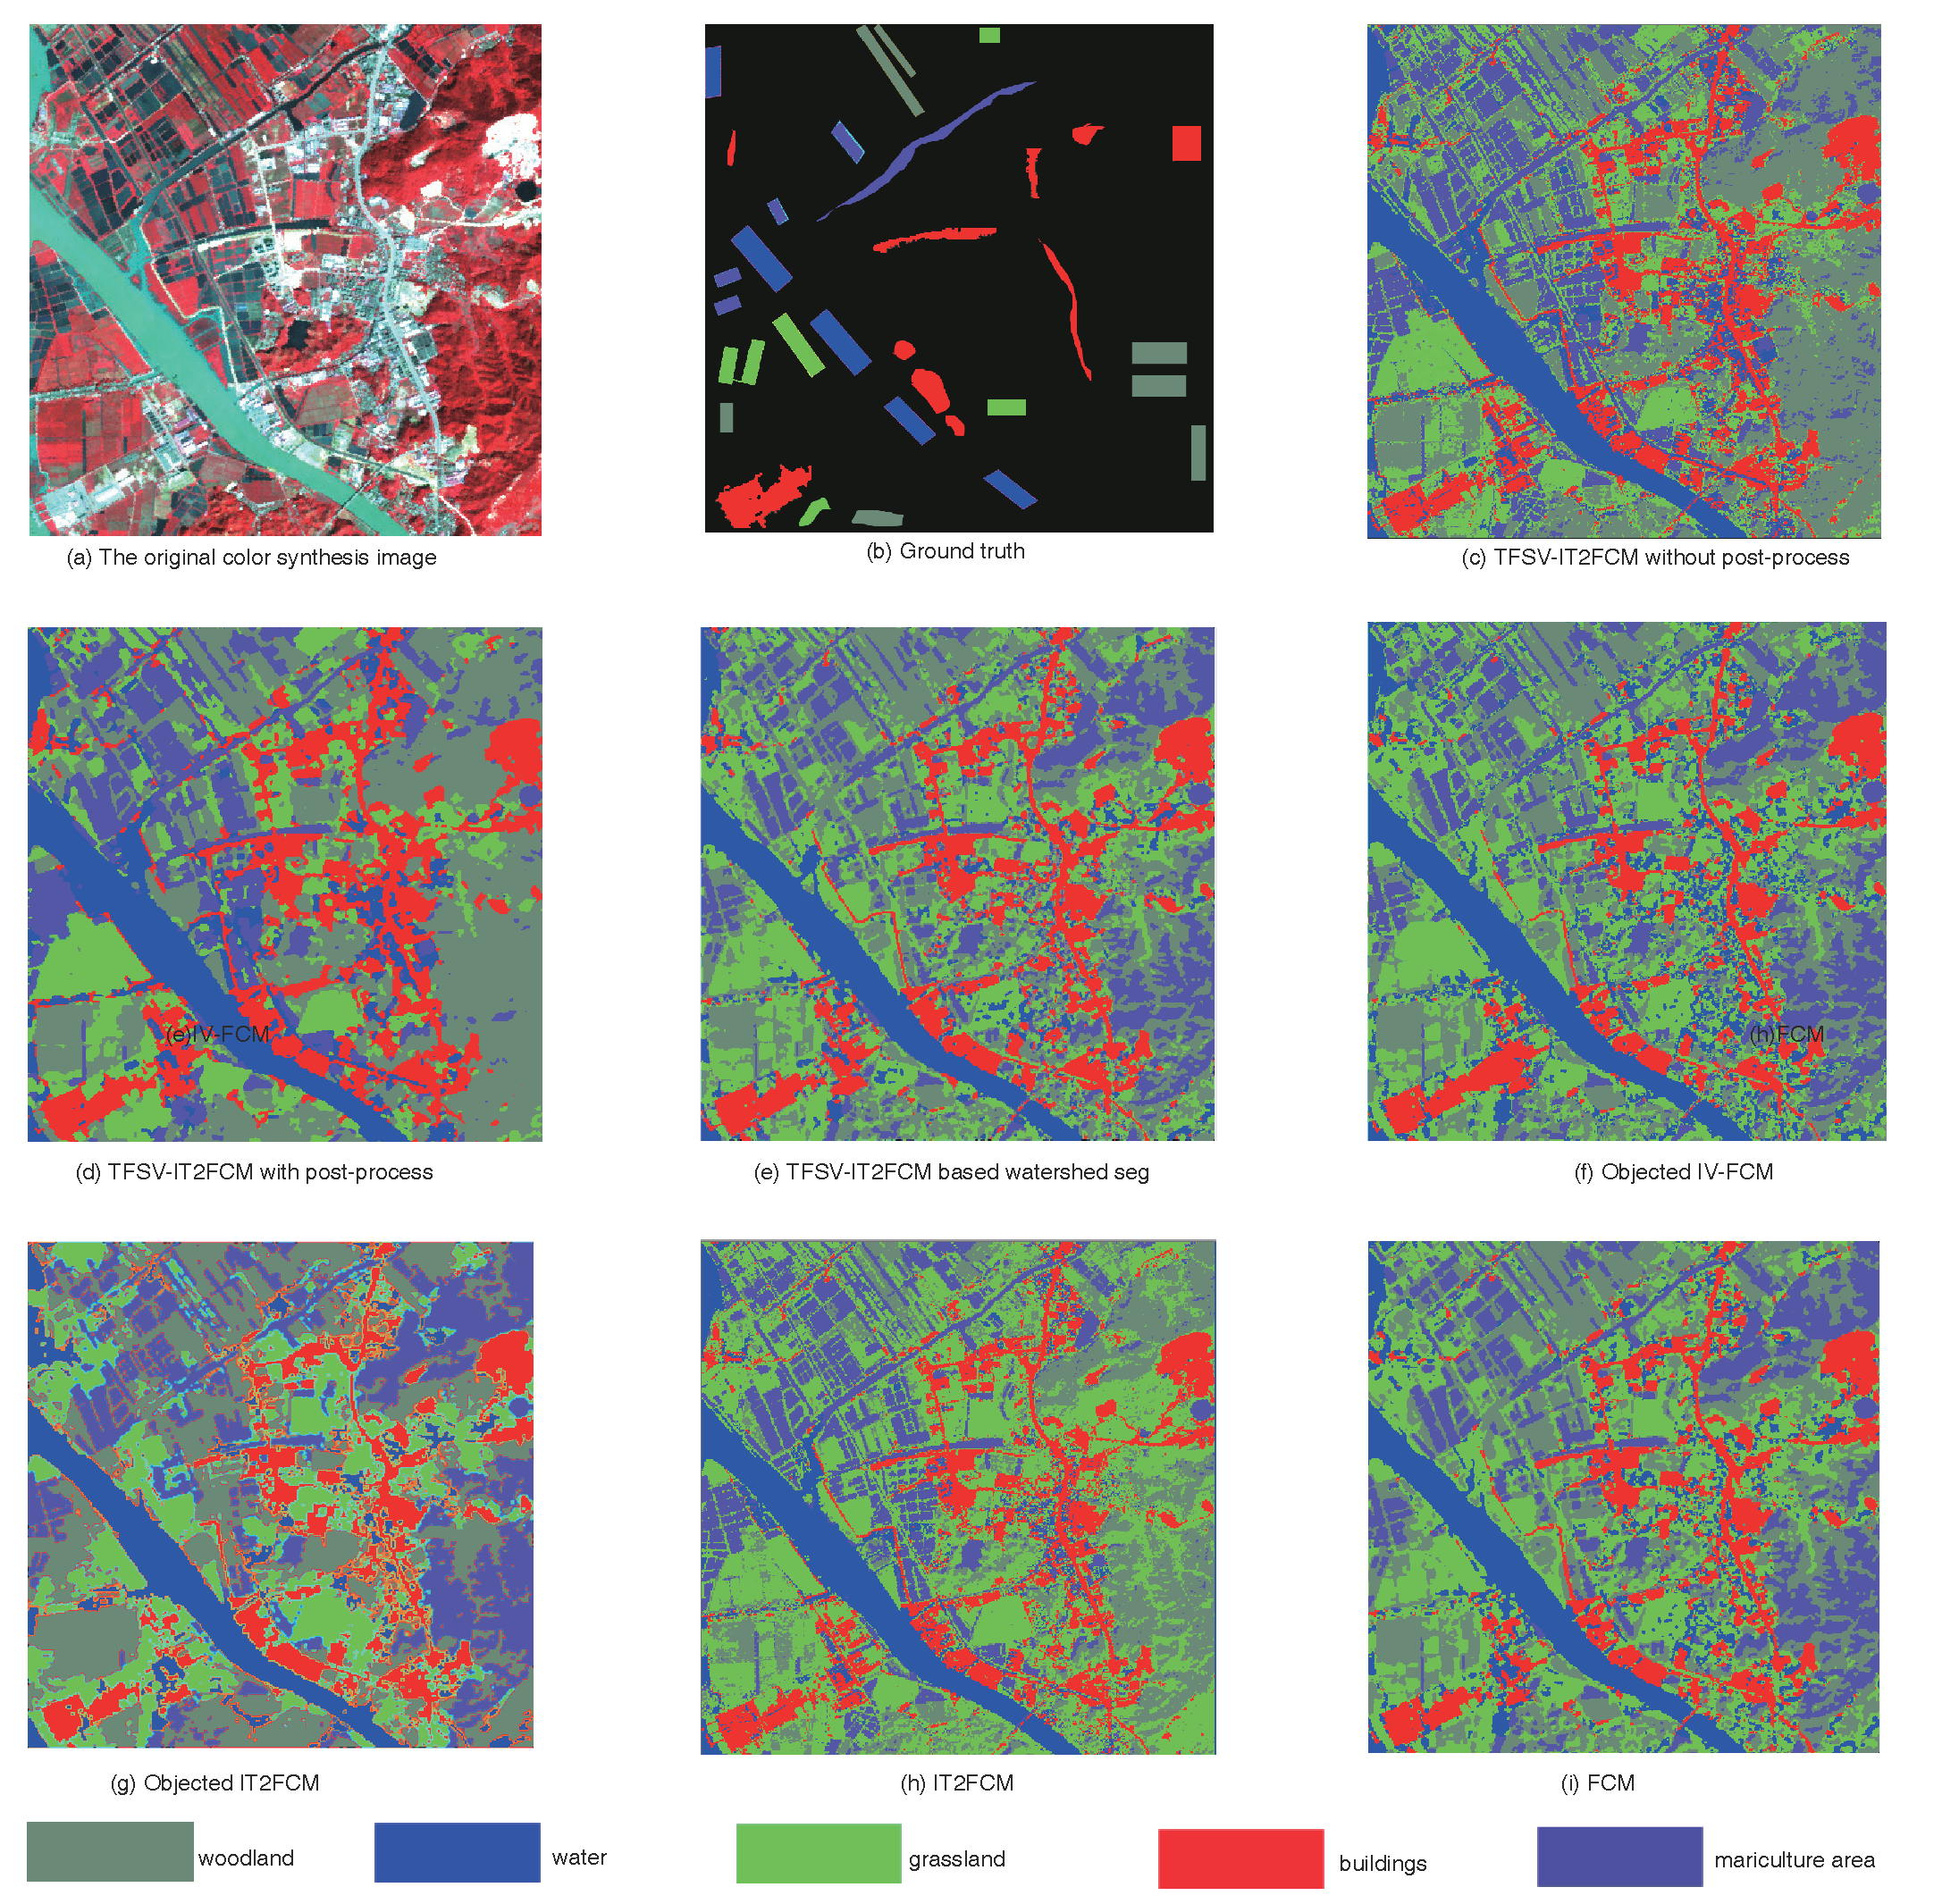
\includegraphics[width=1.0\textwidth]{figures/shenwan}
    \caption{神湾研究区不同方法分类结果示意图 }\label{fig:shenwan}
\end{figure}

\subsection{神湾地区实验}
\label{subsec::chap03-4-1}
神湾研究区位于广东省中山市境内,是一个复杂的种植区域,该区域的高分影像由SPOT 5 遥感卫星于2008 年拍摄。SPOT 5遥感卫星影像包含四个波段,空间分辨率大约$10$ 米,光谱范围$0.4-0.9$ 微米。 神湾地区地物覆被可划分为5大类,分别是:水域、草地、建筑和养殖水域。实验中选择影像$B1$、$B2$、$B3$ 波段合成RGB 图像,如图\ref{fig:shenwan}(a) 所示,其包含$400 \times 400$ 个像素。

在该研究区,文中提出的面向对象的TFSV-IT2FCM 算法分别与其他聚类分割算法进行比较,包含基于像素的聚类方法 (FCM 算法,IT2FCM 算法)和面向对象的聚类方法 (面向对象的IT2FCM, 面向对象的IV-FCM 算法),聚类结果分别由图\ref{fig:shenwan}(f)-(i) 展示。另外,文中提出的TFSV-IT2FCM 算法包含三个主要处理步骤:影像分割,聚类和后处理。图\ref{fig:shenwan}(c) 和\ref{fig:shenwan}(d) 分别展示是否使用后处理的分割结果;图\ref{fig:shenwan}(e) 是获取影像分割单元时使用分水岭分割算法替换SLIC 超像素分割算法得到。通过目视各方法对研究区的聚类分割结果,可以得到以下结论:

\begin{enumerate}[(1)]
    \item 图\ref{fig:shenwan}(c) 和\ref{fig:shenwan}(d) 无论是否使用后处理操作,两者均有大致相似的分割类别区域,图\ref{fig:shenwan}(d) 使用后处理操作具有较少的奇异点。
    \item 图\ref{fig:shenwan}(e) 中使用分水岭算法获取分割单元,与图\ref{fig:shenwan}(d) 相比,一些建筑类别的分割单元被错误划分为草地。因此,获取影像分割单元的分割算法在一定程度上会影像最后聚类分割的精度。
    \item 比较图\ref{fig:shenwan}(f)-(i) 和图\ref{fig:shenwan}(d) 中的聚类计结果可知,这些聚类方法在水域的识别上都有不错的效果。然而,对于IV-FCM 算法(图\ref{fig:shenwan}(f)),一些草地类别被错分为林地类别;对于面向对象的IT2FCM 算法(图\ref{fig:shenwan}(g)),由于建筑、草地和林地这三类有相近的光谱波段,图中左下角区域无法明确区分三者;另外,与面向对象的方法相比,基于像素的IT2FCM 算法和FCM 算法(分别为图\ref{fig:shenwan}(g) 和(h)) 在同类别大区域中产生许多异类别的异常小块。
\end{enumerate}
综上所述,神湾研究区可视化的分类结果图表明文中提出的TFSV-IT2FCM 聚类分割算法相比其他已有算法能获得更好的遥感影像分割结果。

\begin{table}[htb]
    \caption{神湾地区影像地物类别抽样Ground truth表(pixels)}\label{tab:shenwan_data}
    \centering
    \begin{tabular}{ccccc}
        \toprule
        林地  & 水域  & 草地  & 建筑  & 养殖水域 \\
        \midrule
        10124 & 46250 & 15687 & 23697 & 6942     \\
        \bottomrule
    \end{tabular}
\end{table}

为了得到实验中精确量化的聚类结果图,实验中使用CORINE 土地覆被分类系统生成地物类别ground truth 图,如图\ref{fig:shenwan}(b) 所示。表~\ref{tab:shenwan_data} 为神湾研究区各类别地物抽样点数据表。为了对分类结果进行评价,确定分类的精度和可靠性。本实验中使用以下评价指标度量分类效果:
\begin{enumerate}
    \item \textbf{生产者精度(Producer's accuracy, PA)}

          生产者精度是指分类器将整个影像像元正确分为A类的像元数(对角线值)与A类真实像元参考总数的比值。
    \item \textbf{用户精度(User's accuracy, UA)}

          用户精度是指正确分到A类的像元总数(对角线值)与分类器将整个影像的像元分为A类的像元总数(混淆矩阵中A类行的总和)比率。
    \item \textbf{总体分类精度(Overall accuracy, OA)}

          总体分类精度是指所有类别中正确分类的像元总和除以总像元数。
    \item \textbf{Kappa 系数}

          Kappa 系数基于混淆矩阵,用于衡量分类精度。计算公式为
          \begin{equation}\label{eq:kappa}
              \begin{split}
                  Kappa = \frac{\mbox{总体准确度}-\mbox{期望准确度}}{1-\mbox{期望准确度}} = \frac{N\sum_{i=1}^n(X_{ii}) - \sum_{i=1}^n(X_{i+} \times X_{+i})}{N^2 - \sum_{i=1}^n(X_{i+} \times X_{+i})}
              \end{split}
          \end{equation}
\end{enumerate}
式中,$n$ 表示类别,$N$ 表示总类别数,$X_{ii}$ 表示混淆矩阵对角线元素,$X_{+i}$ 表示类别的行总和,$X_{i+}$ 表示类别的列总和。

\begin{table*}[htbp]
    \centering
    \caption{ 神湾研究区不同方法分类精度表}
    \label{tab:shenwan_result}
    \resizebox{\textwidth}{!}{
        \begin{threeparttable}[b]
            \begin{tabular}{cccccccc}
                \toprule
                地物类别                   & TFSV-IT2FCM\tnote{1} & TFSV-IT2FCM\tnote & TFSV-IT2FCM\tnote{2} & IV-FCM & IT2FCM\tnote{2} & IT2FCM\tnote{4} & FCM    \\\cline{1-8}
                \multicolumn{8}{c}{生产者精度 (\%)}                                                                                                                \\
                \midrule
                林地                       & 89.39                & 89.44             & 89.44                & 89.52  & 79.70           & 89.32           & 79.70  \\
                水域                       & 94.08                & 94.58             & 94.18                & 93.59  & 94.06           & 94.09           & 94.21  \\
                草地                       & 83.69                & 84.23             & 84.78                & 79.74  & 81.28           & 77.91           & 80.43  \\
                建筑                       & 87.88                & 88.45             & 88.14                & 88.21  & 87.73           & 83.58           & 81.00  \\
                养殖水域                   & 80.32                & 81.29             & 76.01                & 64.08  & 50.83           & 48.33           & 45.73  \\\cline{1-8}
                \multicolumn{8}{c}{用户精度 (\%)}                                                                                                                  \\\cline{1-8}
                林地                       & 82.98                & 83.39             & 83.39                & 84.10  & 77.46           & 82.40           & 77.46  \\
                水域                       & 95.54                & 97.34             & 97.34                & 97.34  & 95.18           & 92.58           & 90.85  \\
                草地                       & 82.96                & 82.96             & 82.96                & 80.69  & 70.21           & 72.32           & 63.84  \\
                建筑                       & 91.95                & 90.68             & 87.97                & 86.04  & 84.60           & 86.04           & 86.46  \\
                养殖水域                   & 69.27                & 69.27             & 70.71                & 56.31  & 70.71           & 61.93           & 69.27  \\
                \cline{1-8}
                \textbf{总体分类精度 (\%)} & 89.78                & 90.33             & 89.81                & 88.11  & 85.52           & 84.90           & 82.93  \\
                \textbf{Kappa 系数}        & 0.8544               & 0.8621            & 0.8546               & 0.8302 & 0.7954          & 0.7871          & 0.7605 \\
                \bottomrule
            \end{tabular}
            \begin{tablenotes}
                \item[1] {TFSV-IT2FCM 算法,没有做后处理}
                \item[2]{该方法中影像分割阶段使用Watershed 方法获取影像分割单元}
                \item[3]{面向对象的IT2FCM 方法}
                \item[4]{基于像素的IT2FCM 方法}
            \end{tablenotes}

        \end{threeparttable}
    }
\end{table*}

表~\ref{tab:shenwan_result} 为各方法在神湾地区影像上的地物类别识别精度。文中提出的TFSV-IT2FCM 算法获得最好的OA 精度,为$90.33\%$,相比无后处理的TFSV-IT2FCM 算法、基于Watershed 分割的TFSV-IT2FCM 算法、 IV-FCM 算法、面向对象的IT2FCM 算法、基于像素的IT2FCM 算法和FCM 算法分别提升了$0.55\%$、$0.52\%$、$2.22\%$、$4.81\%$、$5.43\%$的分类精度。
分类精度也表明对于文中提出的聚类分割算法,聚类是最重要的一步,在方法的三个部分(分割、聚类、后处理)中最大化的决定最终分类结果精度。Kappa系数结果也表明,文中提出的TFSV-IT2FCM 算法有效题目了影像地物的特征,获得了最佳的聚类分割结果。表中数值量化的结果基本与前文可视化的结果一致。

\begin{figure}[htbp]
    \centering
    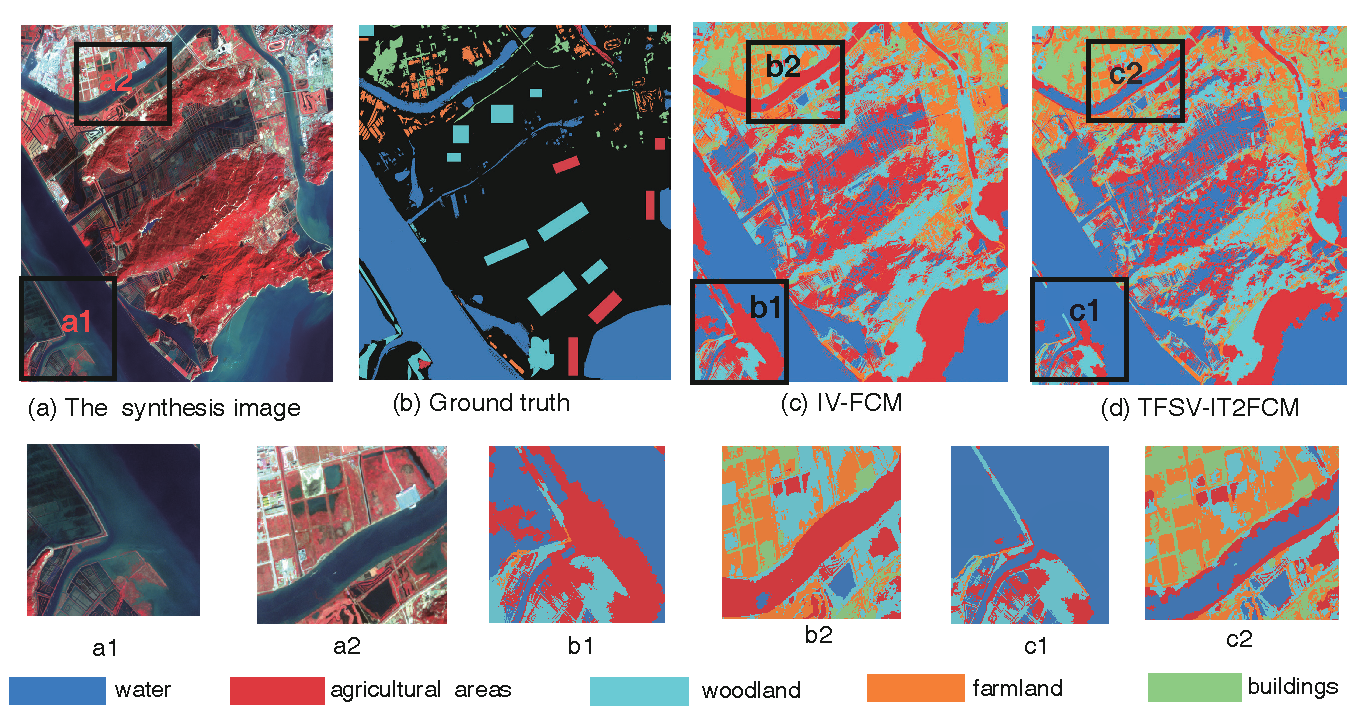
\includegraphics[width=1.0\textwidth]{figures/hengqin}
    \caption{神湾研究区TFSV-IT2FCM 与IV-FCM 算法聚类分割图 }\label{fig:hengqin}
\end{figure}

\subsection{横琴地区实验}
\label{subsec::chap03-4-1}
第二个研究区横琴岛位于广东省珠海市,岛内具有复杂的农业与养殖区,该区域高分影像
由SPOT 5 遥感卫星于2010 年拍摄。横琴地区地物类别可分为水域、农业区、林地、农田和建筑这五大类。实验区选择影像图像如图~\ref{fig:hengqin}(a) 所示,大小为$1203 \times 1055$ 个像素。

在神湾研究区我们比较了文中提出的TFSV-IT2FCM 算法与其他算法的聚类分割结果,初步验证了TFSV-IT2FCM 算法的改进效果。文献\cite{he2016remote} 中证明了IV-FCM 算法相比其他聚类分割算法可以取得更好的实验精度,因此,在横琴地区和三门峡地区的实验中,我们着重比较提出的TFSV-IT2FCM 算法与IV-FCM 算法的实验效果。

IV-FCM 算法和TFSV-IT2FCM 算法的可视化结果分别如图~\ref{fig:hengqin}(c) 和(d) 所示。结合目视解译可知,两种方法对具有明显边界的地物类别都有良好的划分,基本实现同一类地物划分的一致性。 参照图~\ref{fig:hengqin}(b) 中的真实地物分类,对比~\ref{fig:hengqin}(c) 和(d)中可视化结果,可以看出TFSV-IT2FCM算法对于一定范围内不同光谱特征的同一类别具有较大的容忍性。例如,图~\ref{fig:hengqin}(a1) 左上角水域的光谱特征是不均匀的,图~\ref{fig:hengqin}(b1) 和(c1) 结果表明TFSV-IT2FCM 算法将该区域正确划分为水域,由于水域的几个光谱与农业区相近,而IV-FCM 算法则将其错分为农业区。类似地,对于图~\ref{fig:hengqin}(a2)中地物覆被复杂的区域,TFSV-IT2FCM 算法能正确地将水与农田、建筑物等其他地物区分开来,而IV-FCM 算法则存在一定的分类错误。例如,在图~\ref{fig:hengqin}(b2)中,河流中的水被错误地划分为农业区; 然而,在图~\ref{fig:hengqin}(c2)中,TFSV-IT2FCM算法的结果清晰地识别出了河流两岸的水和其他物体。

\begin{table*}[htbp]
    \centering
    \caption{ 横琴地区分类结果表}
    \label{tab:hengqin_result}
    \makebox[\textwidth]{
    \begin{adjustbox}{max width=1.15\textwidth}
        \begin{tabular} {llllllllllllll}
            \toprule
            \multicolumn{1}{l}{\multirow{3}*{{分类结果}}} & \multicolumn{6}{c}{\textbf{TFSV-IT2FCM}} & \multicolumn{6}{c}{\textbf{IV-FCM}}                                                                                                                                                                  \\ \cline{2-13}
                                                          & \multicolumn{5}{l}{采样点}               & \multicolumn{1}{c}{\multirow{2}*{{用户精度(\%)}}} & \multicolumn{5}{l}{采样点} & \multicolumn{1}{c}{\multirow{2}*{{用户精度(\%)}}}                                                                   \\\cline{2-6}  \cline{8-12}\\
                                                          & 水域                                     & 农业区                                            & 林地                       & 农场                                              & 建筑  &       & 水域   & 农业区 & 林地  & 农场  & 建筑  &       \\
            \midrule
            水域                                          & 241231                                   & 10022                                             & 44                         & 0                                                 & 0     & 95.99 & 196301 & 54380  & 557   & 59    & 0     & 78.12 \\
            农业区                                        & 21025                                    & 70848                                             & 4755                       & 57                                                & 1     & 73.28 & 9810   & 78463  & 8338  & 74    & 1     & 81.15 \\
            林地                                          & 1108                                     & 11672                                             & 66320                      & 2167                                              & 18    & 81.59 & 167    & 8971   & 71578 & 569   & 0     & 88.06 \\
            农场                                           & 0                                        & 43                                                & 4032                       & 28234                                             & 724   & 85.47 & 0      & 7      & 10192 & 22785 & 49    & 68.98 \\
            建筑                                          & 0                                        & 0                                                 & 0                          & 1132                                              & 36236 & 96.97 & 0      & 0      & 0     & 4310  & 33058 & 88.47 \\
            合计                                          & 263364                                   & 92585                                             & 75151                      & 31590                                             & 36979 &       & 206278 & 141821 & 90665 & 27797 & 33108 &       \\
            生产者精度(\%)                                & 91.60                                    & 76.52                                             & 88.25                      & 89.38                                             & 97.99 &       & 95.16  & 55.33  & 78.95 & 81.97 & 99.85 &       \\
            \bottomrule
        \end{tabular}
    \end{adjustbox}}
\end{table*}

\begin{figure}[htbp]
    \centering
    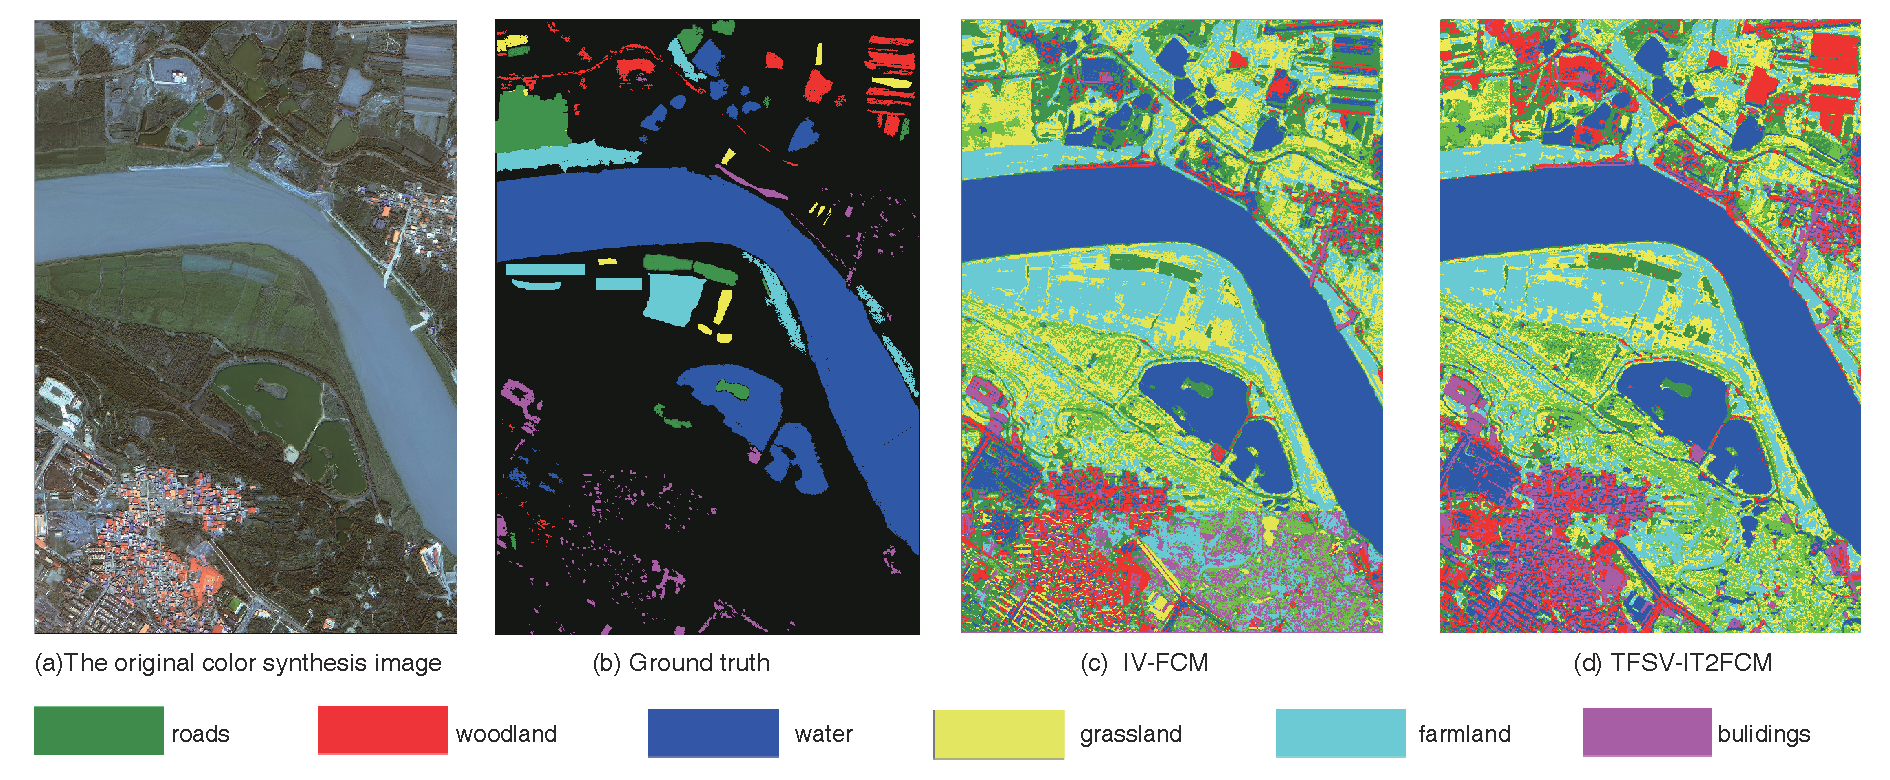
\includegraphics[width=1.0\textwidth]{figures/sanmenxia}
    \caption{三门峡研究区不同方法分类结果示意图 }\label{fig:sanmenxia}
\end{figure}

同样,为了获取横琴地区精确的分类结果,文中使用CORINE 土地分类系统随机采样$499,669$ 个像素点作为ground truth 图,如表~\ref{tab:hengqin_result} 所示,TFSV-IT2FCM 方法中$10,022$ 个像素由“农业区” 被错分为“水域”,而在IV-FCM 方法中被错分的像素点为$54,380$ 个。TFSV-IT2FCM 方法相比IV-FCM 方法,“水域”类别的用户精度从$78.12\%$ 提升到$95.99\%$。 表~\ref{tab:hengqin_result} 中的用户精度和生产者精度也表明TFSV-IT2FCM 聚类方法的性能要比IV-FCM 方法更好。

\begin{table}[htbp]
    \caption{横琴地区分类精度表}\label{tab:hengqin_oa}
    \centering
    \begin{tabular}{llll}
        \toprule
        研究区 & 方法        & OA(\%) & Kappa 系数 \\
        \midrule
        横琴   & TFSV-IT2FCM & 88.63  & 0.8290     \\
               & IV-FCM      & 80.49  & 0.7210     \\
        \bottomrule
    \end{tabular}
\end{table}

表~\ref{tab:hengqin_oa} 中比较了TFSV-IT2FCM 方法和IV-FCM 方法在横琴地区的总体分类精度和Kappa 系数,TFSV-IT2FCM 方法的OA 从$80.49\%$ 提升到$88.63\%$, 同时Kappa 系数由$0.7210$ 提升到$0.8290$。

\subsection{三门峡地区实验}
\label{subsec::chap03-4-1}
神湾地区与横琴地区遥感影像均由SPOT 5 遥感卫星拍摄,为了验证不同卫星影像的聚类分割结果,文中选取高分二号遥感卫星拍摄三门峡地区的遥感影像,影像空间分辨率为$1$ 米。三门峡研究区位于河南省三门峡市,具有复杂的城市地形。实验中选择影像$1$、$2$、$3$ 三个波段合成RGB 图像,如图\ref{fig:sanmenxia}(a) 所示,其包含$1625 \times 2320$ 个像素。


\begin{table*}[htbp]
    \centering
    \caption{三门峡地区分类结果表}
    \label{tab:sanmenxia_result}
    \makebox[\textwidth]{
    \begin{adjustbox}{max width=1.15\textwidth}
        \begin{tabular} {llllllllllllllll}
            \toprule
            \multicolumn{1}{l}{\multirow{3}*{{分类结果}}} & \multicolumn{7}{c}{\textbf{TFSV-IT2FCM}} & \multicolumn{7}{c}{\textbf{IV-FCM}}                                                                                                                                                                                       \\ \cline{2-15}
                                                          & \multicolumn{6}{l}{采样点}               & \multicolumn{1}{c}{\multirow{2}*{{用户精度(\%)}}} & \multicolumn{6}{l}{采样点} & \multicolumn{1}{c}{\multirow{2}*{{用户精度(\%)}}}                                                                                        \\\cline{2-7}  \cline{9-14}\\
                                                          & 道路                                     & 林地                                              & 水域                       & 草地                                              & 农田   & 建筑   &       & 道路  & 林地   & 水域   & 草地   & 农田   & 建筑   &       \\
            \midrule
            道路                                          & 72564                                    & 4598                                              & 0                          & 2965                                              & 368    & 3770   & 86.11 & 62754 & 12385  & 341    & 3169   & 513    & 5103   & 74.47 \\
            林地                                          & 591                                      & 197835                                            & 6542                       & 39638                                             & 456    & 376    & 80.60 & 891   & 176238 & 25324  & 31528  & 301    & 11156  & 71.80 \\
            水域                                          & 0                                        & 0                                                 & 310128                     & 1360                                              & 2436   & 2625   & 97.97 & 0     & 358    & 310524 & 1257   & 2613   & 1797   & 98.10 \\
            草地                                          & 3421                                     & 16329                                             & 865                        & 249431                                            & 405    & 0      & 92.23 & 2598  & 25341  & 516    & 231265 & 5639   & 5092   & 85.51 \\
            农田                                          & 0                                        & 673                                               & 1539                       & 16234                                             & 291035 & 2391   & 93.32 & 0     & 408    & 2538   & 14840  & 289024 & 5062   & 92.67 \\
            建筑                                          & 8589                                     & 23768                                             & 356                        & 3568                                              & 4997   & 283703 & 87.30 & 6589  & 85961  & 0      & 2167   & 3219   & 227045 & 69.86 \\
            合计                                          & 85165                                    & 243203                                            & 319430                     & 313196                                            & 299697 & 292865 &       & 72832 & 300691 & 339243 & 284226 & 301309 & 255255 &       \\
            生产者精度(\%)                                & 85.20                                    & 81.35                                             & 97.09                      & 79.64                                             & 97.11  & 0.97   &       & 86.16 & 58.61  & 91.53  & 81.37  & 95.92  & 88.95  &       \\
            \bottomrule
        \end{tabular}
    \end{adjustbox}}
\end{table*}

高分二号卫星拍摄的三门峡城市中心区域如图~\ref{fig:sanmenxia} 所示,由原始合成图~\ref{fig:sanmenxia}(a) 中可知,建筑、道路与农田交错复杂。与TFSV-IT2FCM 算法相比, IV-FCM 算法无法精确的区分图中右下角区域的建筑、道路与农田类别。图~\ref{fig:sanmenxia}(d) 中可视化结果表明TFSV-IT2FCM 算法对这三类可以产生明确的边界,分割效果更好。

同样地,随机采样$1553556$ 个像素点生成参考ground truth 图,在三门峡地区对六个地物类别上统计生产者精度和用户精度,结果如表~\ref{tab:sanmenxia_result} 所示, TFSV-IT2FCM 算法对“草地” 的用户精度有近$8\%$ 的绝对值提升。其他类别精度数据也有不同幅度的提升。表~\ref{tab:sanmenxia_oa} 中所示TFSV-IT2FCM 算法在三门峡研究区获得的 OA 精度为$90.42\%$ ,捅死Kappa 系数达到$0.8827$ ,整体比IV-FCM 算法提升近$7\%$ 。

\begin{table}[htbp]
    \caption{三门峡地区分类精度表}\label{tab:sanmenxia_oa}
    \centering
    \begin{tabular}{llll}
        \toprule
        研究区 & 方法        & OA(\%) & Kappa 系数 \\
        \midrule
        三门峡 & TFSV-IT2FCM & 90.42  & 0.8827     \\
               & IV-FCM      & 83.48  & 0.7978     \\
        \bottomrule
    \end{tabular}
\end{table}

为验证文中提出的TFSV-IT2FCM 算法的有效性,文中分别在神湾、横琴和三门峡三个研究区进行高分影像模糊聚类的地物分割sh识别实验。与IV-FCM 算法和其他模糊聚类方法比较得到的可视化结果和量化结果均表明文中提出的TFSV-IT2FCM 算法的有效性,其更能区分遥感影像相似光谱不同类别地物的边界。 同时,TFSV-IT2FCM 算法在SPOT 5 影像(神湾和横琴地区)和高分二号影像(三门峡地区)上的聚类分割均能取得一定的识别优势,可见其不受影像数据源的影像。

\section{本章小结}
\label{sec::chap03-5}
本章考虑遥感影像“同物异谱”和“同谱异物”的固有的不确定性,创新性的定义TFSV 的数据模型来提取影像分割单元的内在特征,同时针对该数据模型提出一种新的模糊集间的区间距离来刻画两个三角形模糊集之间的相似性。并提出TFSV-IT2FCM 算法改进现有面向对象的遥感影像模糊聚类分割方法。分别在SPOT 5影像和高分二号影像上进行地物聚类分割实验,实验可视化结果和数值量化结果均证明了文中提出的TFSV-IT2FCM 算法的有效性,其确实能更好刻画遥感影像数据的不确定性,实现更好的分割识别结果。
